    \documentclass[letterpaper, 10 pt, conference]{ieeeconf}
    
    % ICRA / IEEE conference formatting
    \IEEEoverridecommandlockouts
    \overrideIEEEmargins
    
    % Keep the original citation commands (e.g., \\citep) while using numeric IEEE-style citations.
    % ieeeconf/IEEEtran defines a fake \NAT@parse for hyperref compatibility;
    % undefine it before loading natbib so that \citep and \citet work normally.
    \makeatletter
    \let\NAT@parse\undefined
    \makeatother
    \usepackage[numbers,sort&compress]{natbib}
    
    \usepackage[utf8]{inputenc}
    \usepackage[T1]{fontenc}
    \usepackage{courier}
    \usepackage[hidelinks,hypertexnames=false]{hyperref}
    \usepackage{url}
    \usepackage{booktabs}
    \usepackage{amsmath}
    \usepackage{amsfonts}
    \usepackage{graphicx}
    \usepackage{float}
    \usepackage{microtype}
    \usepackage{xcolor}
    \usepackage{placeins}
    \usepackage{adjustbox}
    \usepackage{multirow}
    
    
    \newcommand{\method}{SafeVantage}
    \newcommand{\hmthree}{HM3D-Sem}
    \newcommand{\support}{\mathrm{support}}

    
    \newcommand{\taskitem}[2]{%
       \item \texttt{#1}: #2%
     }
    
    \title{\LARGE \bf
    \method: Vantage-Aware Memory for Reliable Embodied Decisions
    }
    
    \author{Anonymous Author(s)}
    
    \usepackage{graphicx}
    \usepackage{etoolbox}
    \usepackage{caption}

    \captionsetup[table]{
      name=TABLE,
      position=top,
      format=plain,
      labelsep=period,
      justification=justified,
      singlelinecheck=false,
      font=normalsize,
      labelfont=normalfont,
      textfont=normalfont,
      skip=3pt
    }
    \newif\ifSVteaserregistered
    \SVteaserregisteredfalse    
    
    \makeatletter
    \apptocmd{\@maketitle}{%
        \par
        \vspace{1.0em}
    
        % Register this teaser as Figure 1
        \ifSVteaserregistered
        \else
            \refstepcounter{figure}
            \label{fig:framework}
            \global\SVteaserregisteredtrue
        \fi
    
        \begin{center}
            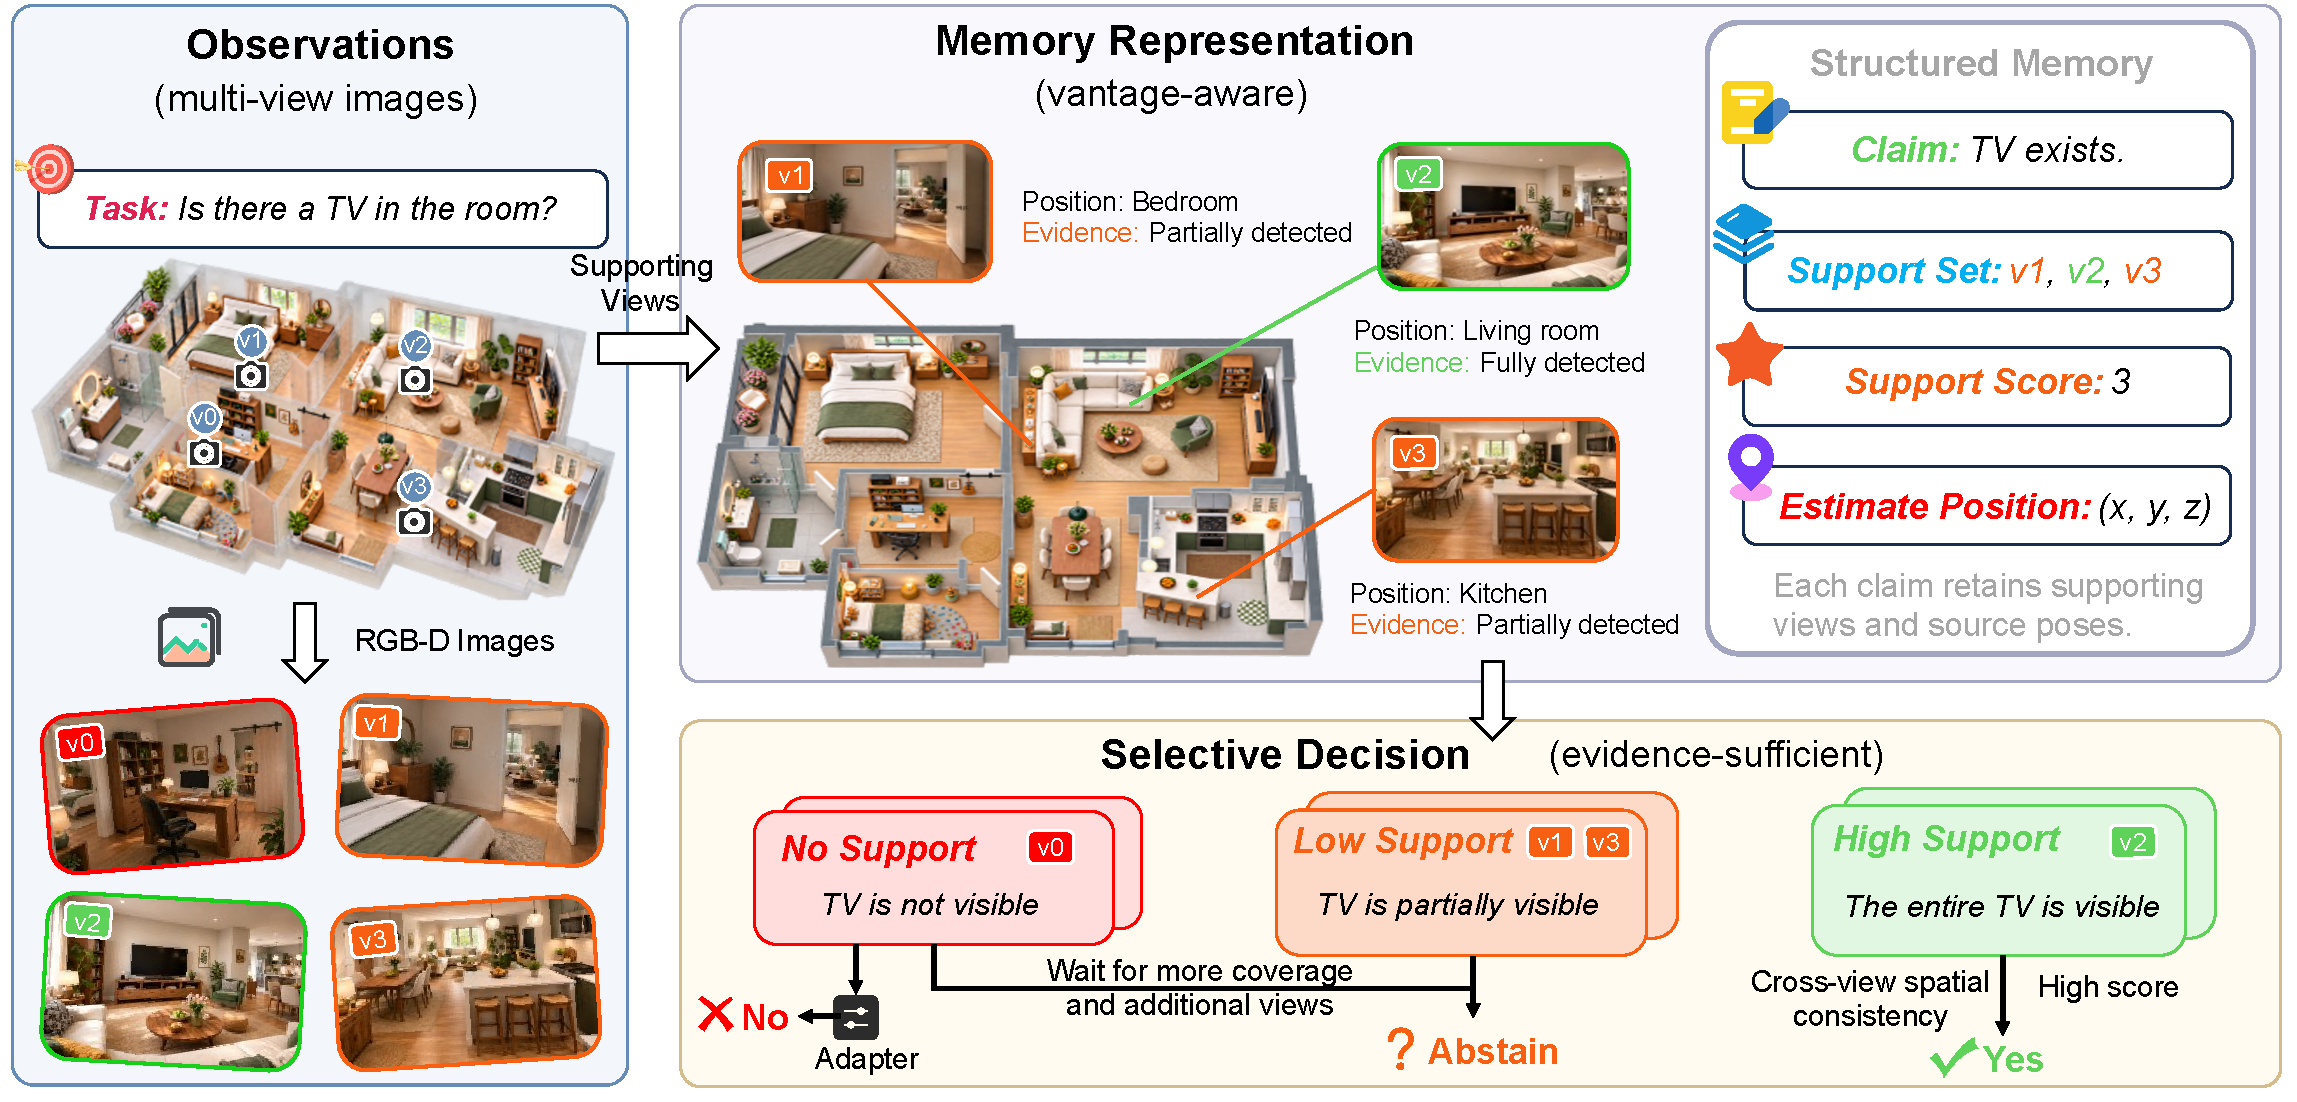
\includegraphics[
                width=0.96\textwidth
            ]{figures/zuyi_figure/framework_v2.pdf}
    
            \vspace{0.3em}
    
            {\normalfont\normalsize
            \captionof*{figure}{%
            Fig.~\thefigure.\textbf{
            Overview of \method{}}, a vantage-aware memory for reliable embodied decisions. It retains the viewpoints that support each claim and uses the evidence to select the next view and make the final \textsc{Yes}/\textsc{No}/\textsc{ABSTAIN} decisions.
            }}
        \end{center}
    
        \vspace{0.8em}
    }{%
    }{%
        \PackageWarning{teaser}{Failed to modify \string\@maketitle}
    }
    \makeatother
    
    
    \begin{document}
    
    \maketitle
    \thispagestyle{empty}
    \pagestyle{empty}
    
    
\begin{abstract}
Reliable embodied decisions under partial observability require informative observations and sufficient supporting evidence. However, semantic scores alone do not reveal which viewpoints justify a claim or where additional evidence should be acquired. We introduce \method{}, a vantage-aware semantic memory and active acquisition framework that retains each claim's supporting views, camera poses, and estimated target location, keeping positive support distinct from search coverage. A learned candidate-observability model uses claim-grounded geometry to predict target visibility at reachable viewpoints. These predictions guide view selection through expected reduction in terminal decision loss, accounting for travel cost and geometrically distinct corroboration. A calibrated head then combines support, spatial consistency, and coverage to produce \textsc{Yes}, \textsc{No}, or \textsc{Abstain} decisions. We evaluate \method{} on a category-presence benchmark spanning 232 unseen ProcTHOR houses and 7,424 paired episodes per method and action budget. Compared with validation-selected equal-budget baselines, \method{} achieves macro-F1 gains of 24.7\% and 12.0\% at eight and twelve actions, respectively, with lower risk and higher answer rates at both budgets and 31.7\% less travel at eight actions. Equal-input HM3D experiments show lower selective risk under fixed observations, while controlled ScanNet interventions show that restoring supporting views improves downstream VLM answers. Ablations further support the contribution of candidate observability to decision quality and acquisition efficiency. Results demonstrate the value of claim-level viewpoint evidence for connecting semantic memory, active acquisition, and reliable decision-making.
\end{abstract}
    
    %\begin{figure}[t]
    %  \centering
    %  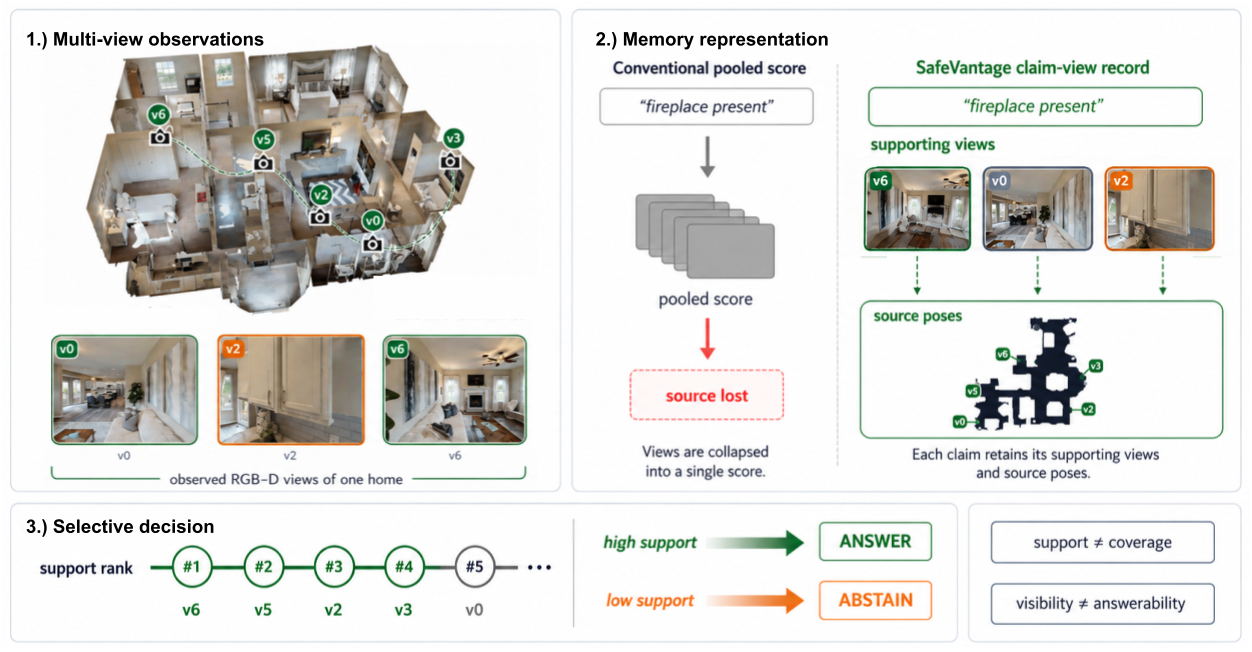
\includegraphics[width=\linewidth]{figures/heyefig1.png}
    %  \caption{\textbf{\method{} links semantic claims to supporting views.} The policy uses the same evidence state to choose the next view and the final \textsc{Yes}/\textsc{No}/\textsc{Abstain} decision.}
    %  \label{fig:teaser}
    %\end{figure}
    
    
    \section{Introduction}
    
    Embodied agents increasingly rely on spatial memory to reason about
    objects and answer questions in partially observed environments.
    OpenScene, VLMaps, and ConceptGraphs connect language with persistent
    2D or 3D scene representations~\citep{peng2023openscene,
    huang2023vlmaps,gu2024conceptgraphs}, while recent EQA systems combine
    memory, exploration, and foundation models for embodied
    reasoning~\citep{das2018embodied,majumdar2024openeqa,exploreeqa2024}.
    However, reliable decision-making requires more than retrieving a likely
    semantic match. The memory must also indicate whether the available observations
    actually provide sufficient evidence for that claim.

    Existing approaches organize multi-view observations into maps, graphs, or selected snapshots~\citep{huang2023vlmaps,gu2024conceptgraphs,yang2024threedmem}. These representations support retrieval, but a semantic score alone does not reveal which viewpoints support a claim, whether they are spatially distinct, or how clearly the target was observed. These differences matter under partial observability: a single weak detection provides different evidence from corroborated observations, while missing detections may reflect incomplete search coverage rather than true absence. Embodied systems have used confidence to stop exploration or request help~\citep{geifman2019selectivenet,cheng2025efficienteqa}. These limitations motivate a claim-level evidence representation that preserves supporting observations, uses their provenance to guide subsequent acquisition, and distinguishes insufficient evidence from evidence of absence through selective abstention.

    In this work, we propose \method{}, a vantage-aware semantic memory that associates each claim with its supporting views, estimated target location, and unresolved evidence. The same evidence state drives the acquisition-to-decision loop: the policy explores for relevant evidence, uses claim-grounded target geometry to predict the observability of candidate views, and uses supporting-view provenance to seek geometrically distinct corroboration. The accumulated evidence then yields a selective \textsc{Yes}, \textsc{No}, or \textsc{Abstain} decision, distinguishing insufficient observation from evidence of absence. Fig.~\ref{fig:framework} illustrates the overview of \method{}.
    We evaluate \method{} on an active-view benchmark constructed from the official ProcTHOR-10K splits~\citep{deitke2022procthor}. Across 232 unseen houses and 7,424 paired episodes per method and action budget, \method{} improves macro-F1 and reduces decision risk against the strongest equal-budget baselines at both action budgets, while also reducing travel. We further isolate the role of vantage-aware evidence through equal-input HM3D comparisons, controlled ScanNet view-removal interventions, and component ablations.
    
    Our main contributions are summarized as follows:
    \begin{enumerate}
        \item We introduce \method{}, a vantage-aware semantic memory that
        preserves claim-level viewpoint provenance, target localization, and
        unresolved evidence instead of collapsing multi-view observations into
        a single semantic score.
    
        % \item We develop an evidence-guided active acquisition framework that
        % uses the same memory state to explore for missing evidence, corroborate
        % provisional detections, and make selective \textsc{Yes}/\textsc{No}/
        % \textsc{ABSTAIN} decisions.

        \item We develop a claim-conditioned active acquisition framework in which
        retained target geometry predicts candidate-view observability, while
        supporting-view provenance guides geometrically distinct corroboration
        before selective \textsc{Yes}/\textsc{No}/\textsc{ABSTAIN} decisions.
    
        \item We establish a ProcTHOR active-view evaluation with 5
        equal-budget acquisition baselines on which \method{} attains the best risk, macro-F1, and answer rate at both action budgets, complemented by HM3D equal-input evaluation, ScanNet interventions, and component ablations.
    \end{enumerate}

\begin{figure*}[t]
\centering
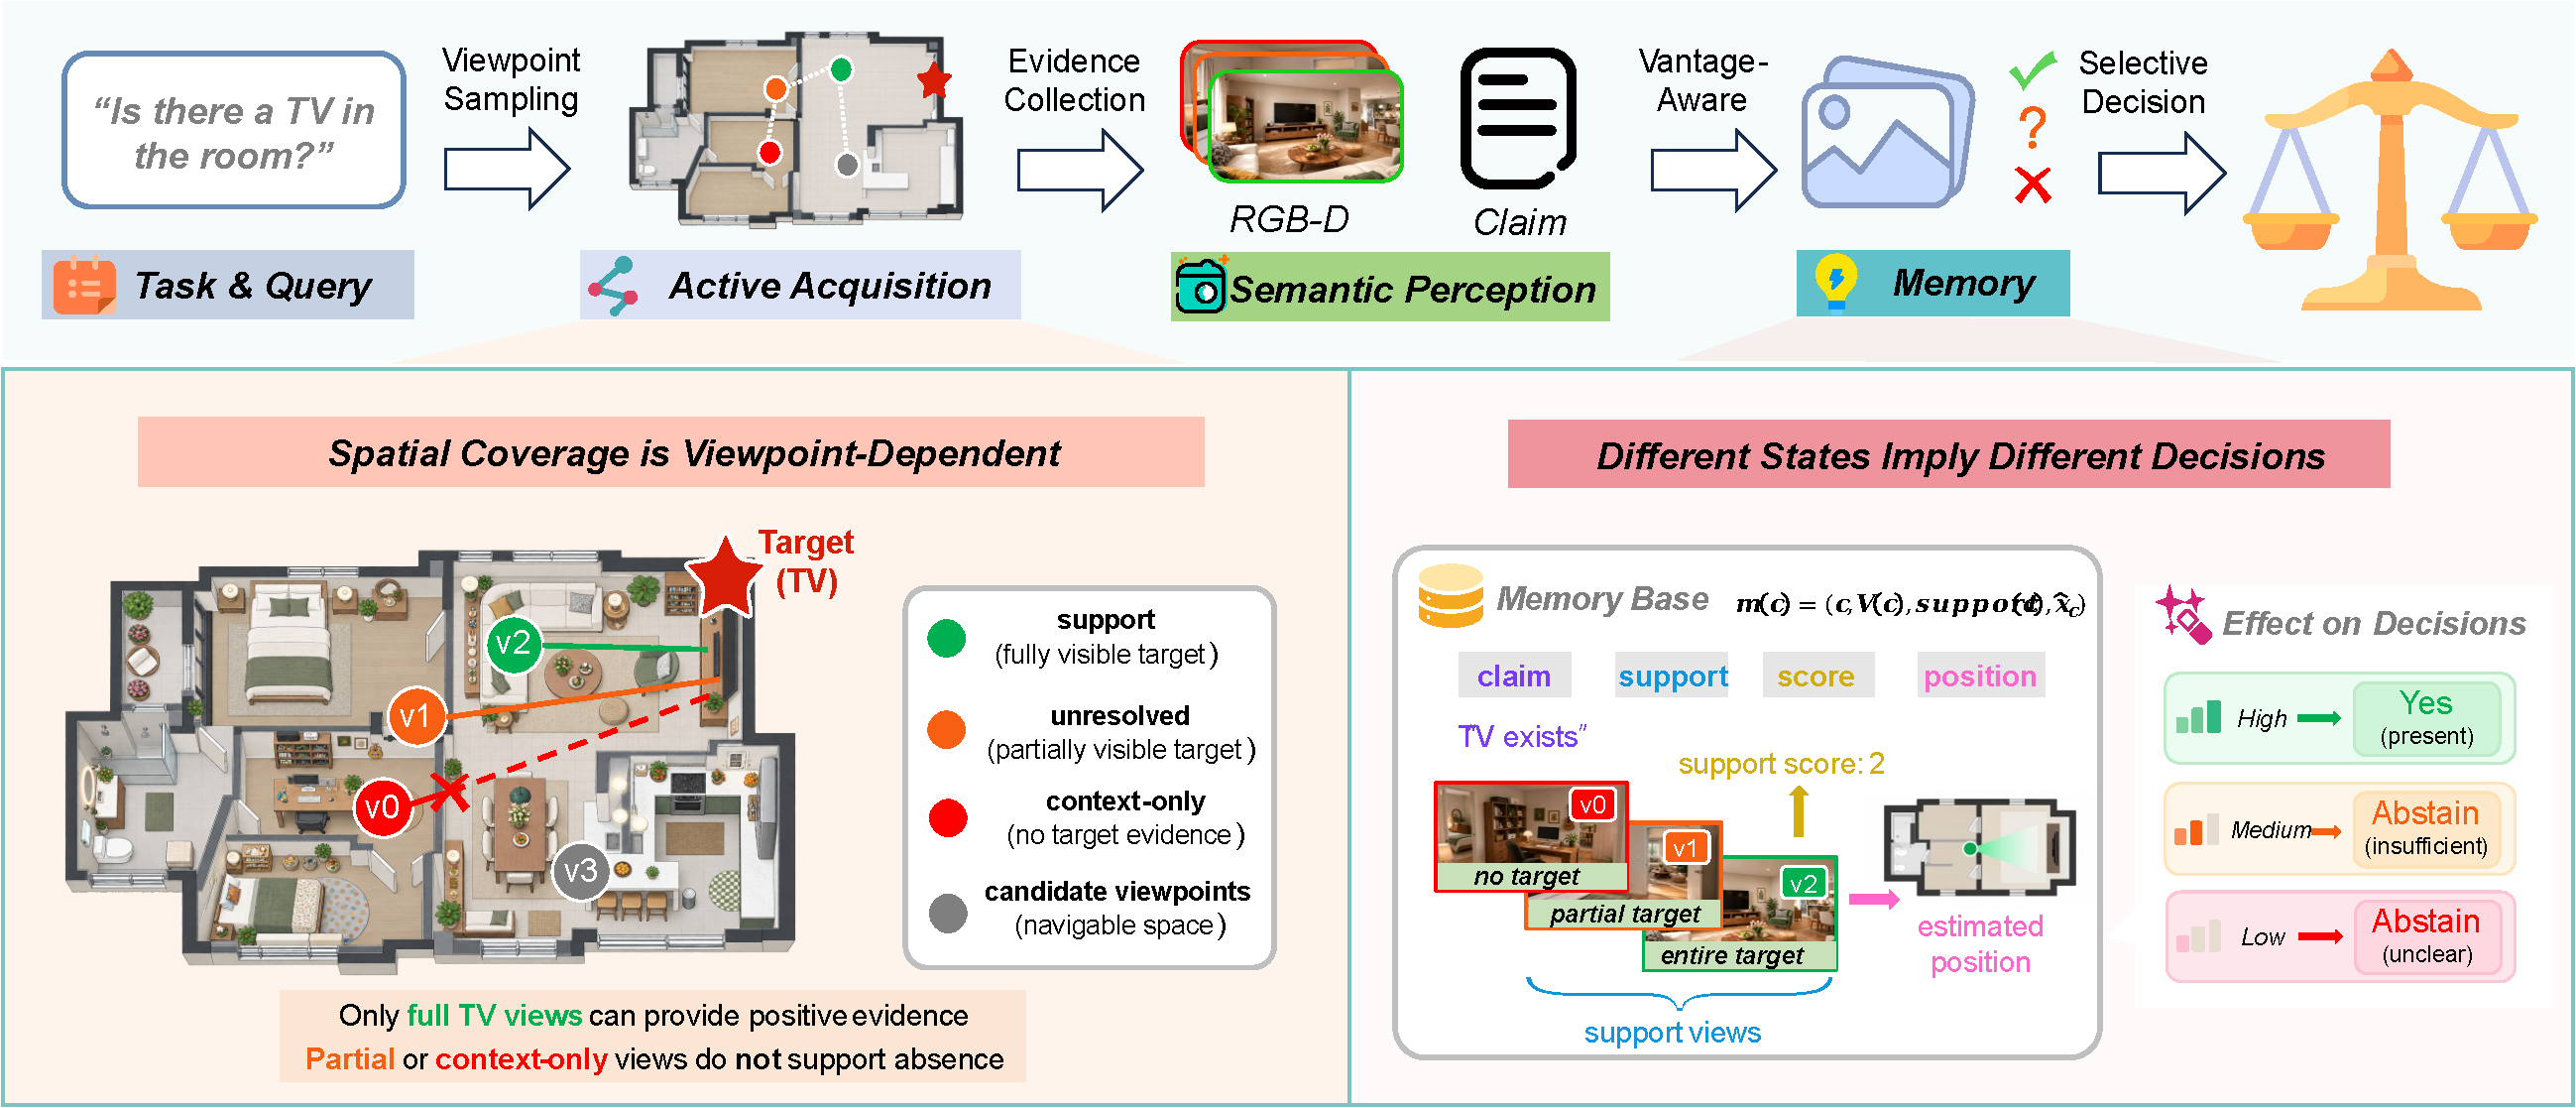
\includegraphics[width=0.96\textwidth]{figures/zuyi_figure/method.pdf}
\caption{\textbf{Viewpoint support and search coverage provide complementary evidence.} Navigable viewpoints differ in the target evidence they reveal. Supporting observations provide positive evidence, whereas partial or context-only observations do not justify absence. Retained views and target geometry inform subsequent acquisition and selective decisions.}
\label{fig:coverage}
\end{figure*}
    
    
\section{Related Work}

\subsection{Open-vocabulary Spatial Memory}

Open-vocabulary spatial representations connect language with scene geometry for semantic retrieval and navigation. VLMaps and OpenScene associate vision--language features with 2D maps and dense 3D geometry~\citep{huang2023vlmaps,peng2023openscene}, while LERF embeds language into radiance fields~\citep{kerr2023lerf}. ConceptGraphs and OpenVoxel organize observations into object-centric graphs and captioned voxel groups~\citep{gu2024conceptgraphs,huang2026openvoxel}. HOV-SG introduces floor--room--object hierarchies for navigation~\citep{werby2024hierarchical}, and FARM combines relational memory with viewpoint evidence~\citep{he2026farm}. These methods support semantic localization and retrieval, with some also retaining source observations. Rather than proposing another mapping backbone, \method{} uses claim-level viewpoint provenance for both active acquisition and selective decisions. ConceptGraphs and VLMaps serve as map-centric alternatives in our equal-input evaluation.

\subsection{Embodied Question Answering and Exploration}

EQA requires agents to collect and integrate observations under partial observability~\citep{das2018embodied}. OpenEQA benchmarks episodic and active answering, Explore-EQA calibrates exploration stopping, and EfficientEQA studies efficient open-vocabulary answering~\citep{majumdar2024openeqa,exploreeqa2024,cheng2025efficienteqa}. MemoryEQA, GraphEQA, and 3D-Mem organize observation histories, semantic scene graphs, and informative snapshots for retrieval and reasoning~\citep{memoryeqa2025,saxena2025grapheqa,yang2024threedmem}. EXPRESS-Bench evaluates exploration-grounded answers, while Mind Palace studies long-term active EQA with structured memory and value-of-information stopping~\citep{jiang2025express,ginting2025mindpalace}. DAAAM and UQ-DAAAM extend memory to dynamic scenes and uncertainty-aware refinement~\citep{gorlo2025daaam,zhang2026uqdaaam}. These approaches improve memory construction, retrieval, and exploration for answering questions. Our work focuses on category-presence decisions and uses each claim's supporting observations to guide further acquisition and assess whether a decision is sufficiently supported.

\subsection{Active Perception and View Selection}

Active perception selects observations to obtain task-relevant information. For semantic navigation, SemExp learns goal-oriented exploration from episodic semantic maps~\citep{chaplot2020object}, while PONI predicts potential functions over semantic maps to guide object search~\citep{ramakrishnan2022poni}. VLFM uses vision--language value maps for frontier selection~\citep{yokoyama2024vlfm}, and SG-Nav combines online 3D scene graphs and LLM reasoning with re-perception to address unreliable detections~\citep{yin2024sg}. These methods use semantic information to direct exploration and verify targets.
% \method{} conditions acquisition on claim-specific supporting views: it explores low-cost or category-relevant regions before detection, then seeks geometrically distinct, target-aligned views for corroboration.
\method{} conditions acquisition on a claim-grounded evidence state: retained target geometry predicts candidate observability, and candidate views are selected according to expected reduction in terminal decision loss.
Our equal-budget baselines isolate coverage-driven, room-prior, and detector-confidence-guided acquisition rather than reproduce these complete navigation systems.

\subsection{Selective Prediction and Abstention}

Selective prediction introduces a reject option to trade coverage against prediction risk~\citep{geifman2019selectivenet, huang2026knowledge}. In robotics, KnowNo uses conformal prediction to determine when a planner should request assistance under ambiguity~\citep{ren2023knowno}. Explore-EQA calibrates exploration stopping~\citep{exploreeqa2024}, while AbstainEQA evaluates abstention when perceptual evidence is unavailable or underspecified~\citep{wu2026abstaineqa}. UQ-DAAAM further incorporates cross-view semantic uncertainty into memory refinement~\citep{zhang2026uqdaaam}. \method{} shares the abstention objective but focuses on the evidence supplied to the decision rule: supporting viewpoints and their spatial consistency remain explicit, while search coverage is represented separately from positive support. Controlled view-removal and restoration experiments further test how access to supporting evidence affects downstream VLM answers.



\section{Method}
\label{sec:method}

We consider category-presence queries under partial observability. Given a claim $c$, \method{} acquires observations within a fixed action horizon $B$ and a geodesic travel budget, then returns \textsc{Yes}, \textsc{No}, or \textsc{Abstain}. The framework comprises semantic memory, active acquisition, and selective decisions.


\subsection{Vantage-aware Semantic Memory}
\label{sec:vantage_memory}

% At viewpoint $v_i$, the agent obtains an observation $o_i=(I_i,D_i,T_i,\tau_i)$ containing RGB, optional depth, camera pose, and timestamp. Let $H_t$ denote the observation history and $\delta_i(c)\in\{0,1\}$ indicate whether the perception adapter reports claim $c$. The supporting viewpoints and their count are
% \begin{equation}
% \begin{aligned}
% V_t(c) &= \{v_i \mid o_i\in H_t,\ \delta_i(c)=1\},\\
% \support_t(c) &= |V_t(c)|.
% \end{aligned}
% \label{eq:support_set}
% \end{equation}
% Each supporting viewpoint retains its source observation and camera pose. When depth is available, back-projection provides per-view target estimates $\hat{\mathbf{x}}_c^{(i)}$ and an approximate aggregate location $\hat{\mathbf{x}}_{c,t}$. The memory record is
% \begin{equation}
% m_t(c)=\big(c,V_t(c),\support_t(c),\hat{\mathbf{x}}_{c,t}\big),
% \label{eq:memory_record}
% \end{equation}
% where the target location is optional.
At viewpoint $v_i$, the agent obtains an observation $o_i=(I_i,D_i,T_i,\tau_i)$ containing RGB, optional depth, camera pose, and timestamp. Let $H_t$ denote the observation history and $\delta_i(c)\in\{0,1\}$ indicate whether the perception adapter reports claim $c$. The supporting viewpoints are $V_t(c)=\{v_i \mid o_i\in H_t,\ \delta_i(c)=1\}$ with support count $\support_t(c)=|V_t(c)|$. Each supporting viewpoint retains its source observation and camera pose. When depth is available, back-projection provides per-view target estimates $\hat{\mathbf{x}}_c^{(i)}$ and an approximate aggregate location $\hat{\mathbf{x}}_{c,t}$. The memory record is $m_t(c)=(c,V_t(c),\support_t(c),\hat{\mathbf{x}}_{c,t})$, where the target location is optional. Because the consistency gate (Eq.~\ref{eq:pair_gate}) accepts only pairs of per-view estimates within radius $r$, detections of instances separated by more than $r$ cannot corroborate one another. The estimate $\hat{\mathbf{x}}_{c,t}$ summarizes the supporting detections by their scores and is used to score candidate views; it does not assume a unique object instance. Support is adapter-specific: ProcTHOR uses YOLO-World scores and boxes~\citep{cheng2024yoloworld}, while HM3D uses Qwen2-VL-7B per-view object lists~\citep{wang2024qwen2vl}. Simulator semantics are not queried by the test-time policy; target visibility is additionally used as a training target for the candidate-observability model. Support counts record detections; their spatial diversity and geometric agreement are assessed separately.

Target visibility, property or relation sufficiency, search coverage, and answer correctness are distinct. For category presence, supporting detections provide positive evidence, whereas missing support may reflect incomplete observation rather than absence (Fig.~\ref{fig:coverage}). Coverage therefore enters the decision features separately from support. Retained source observations also enable the controlled ScanNet interventions described in the experiments.



% \subsection{Claim-conditioned Active Acquisition}
% \label{sec:active_acquisition}

% Let $\mathcal{A}_t$ contain unvisited viewpoints reachable within the remaining geodesic budget, and let $d_t(a)$ denote the incremental travel distance to candidate $a$ in meters.


% Before a provisional detection, the exploration branch balances spatial novelty, category--room evidence, and travel cost. After detection, the corroboration branch scores candidates using the target estimate and existing supporting views:
% \begin{equation}
% \begin{aligned}
% U_t(a;c) &= \frac{G_{\mathrm{corr}}(a)+\lambda_r G_{\mathrm{ray}}(a)}{(0.5+d_t(a))^p}\\
% &\quad+\lambda_c G_{\mathrm{cov}}(a),\\
% a_t^* &= \arg\max_{a\in\mathcal{A}_t} U_t(a;c).
% \end{aligned}
% \label{eq:view_selection}
% \end{equation}
% All gains are conditioned on $H_t$ and $c$. $G_{\mathrm{corr}}$ combines target proximity with distinct-position and yaw diversity; $G_{\mathrm{ray}}$ rewards cameras facing the score-weighted grounded target estimate; and $G_{\mathrm{cov}}$ rewards additional coverage. The weights $\lambda_r,\lambda_c$ balance these terms, while $p$ controls the travel penalty.

% A local edge-length cap limits travel around provisional detections. The eight-action configuration emphasizes low-cost novelty, whereas the twelve-action configuration allows broader coverage. Parameters are selected on training and nested validation scenes and frozen for testing. Each acquired observation updates the history and memory before the next selection.

\subsection{Claim-conditioned Active Acquisition}
\label{sec:active_acquisition}

Let $\mathcal{A}_t$ contain unvisited viewpoints reachable within the
remaining geodesic budget, and let $d_t(a)$ denote the incremental
geodesic travel distance to candidate $a$ in meters.

% For each candidate $a$, \method{} predicts whether the target is likely
% to be observable from that viewpoint. We form a geometric feature vector
% $\psi_t(a,c)$ from the current claim state and candidate geometry,
% including distance to the estimated target, heading alignment, and a
% geodesic baseline feature. The features are standardized using statistics
% frozen from the training scenes, and a logistic outcome model gives
% \begin{equation}
% \hat{o}_t(a,c)
% =
% \sigma\!\left(
% \boldsymbol{\theta}^{\top}\tilde{\psi}_t(a,c)+b_o
% \right),
% \label{eq:observability}
% \end{equation}
% where $\tilde{\psi}_t(a,c)$ denotes the standardized feature vector.
% The outcome model is fit only on training scenes using target
% observability as its training target.

% At test time, the selector receives the acquired controlled-sensor
% observations, the resulting claim state, and candidate geometry. Oracle
% visibility, simulator instance identity, and test labels are not queried
% by the selector.

% Candidate views are selected by their expected reduction in terminal
% decision loss. Let $\hat{p}_t$ be the calibrated belief that claim $c$
% holds given the current top supporting score. A candidate returns either
% a positive reading ($+$) or a null reading ($-$); under the outcome model
% the positive-reading probability is
% \begin{equation}
% p_t^{+}(a,c)=\hat{p}_t\,\hat{o}_t(a,c)+(1-\hat{p}_t)\,\phi,
% \label{eq:reading_prob}
% \end{equation}
% where $\phi$ is a fixed detector false-positive rate. Each outcome induces
% a Bayes posterior over $c$,
% $q_t^{+}=\hat{p}_t\hat{o}_t/p_t^{+}$ and
% $q_t^{-}=\hat{p}_t(1-\hat{o}_t)/(1-p_t^{+})$, and a hypothetical evidence
% state $H_t^{+}$ (a grounded supporting view) or $H_t^{-}$ (a null reading),
% formed with the same online update used at execution. For a decision
% $y\in\{\textsc{Yes},\textsc{No},\textsc{Abstain}\}$ under belief $q$, the
% terminal loss $\ell(y,q)=5(1-q)\mathbf{1}[y{=}\textsc{Yes}]
% +2q\,\mathbf{1}[y{=}\textsc{No}]+0.5\,\mathbf{1}[y{=}\textsc{Abstain}]$
% matches the risk in Eq.~\ref{eq:risk_cost}. Applying the same selective
% rule $\pi_{\mathrm{active}}$ (Eq.~\ref{eq:active_decision}) to each
% hypothetical state gives
% \begin{equation}
% \bar{L}_t(a;c)=
% p_t^{+}\,\ell\!\big(\pi_{\mathrm{active}}(H_t^{+}),q_t^{+}\big)
% +(1-p_t^{+})\,\ell\!\big(\pi_{\mathrm{active}}(H_t^{-}),q_t^{-}\big),
% \label{eq:expected_loss}
% \end{equation}
% and $L_t(c)=\ell(\pi_{\mathrm{active}}(H_t),\hat{p}_t)$ is the loss with no
% further acquisition. The candidate utility is
% \begin{equation}
% U_t(a;c)
% =
% \frac{
% L_t(c)-\bar{L}_t(a;c)-\lambda_d d_t(a)
% }{
% 0.5+d_t(a)
% },
% \label{eq:view_utility}
% \end{equation}
% with $\lambda_d=0.001$. The next viewpoint is
% \begin{equation}
% a_t^*
% =
% \arg\max_{a\in\mathcal{A}_t} U_t(a;c).
% \label{eq:view_selection}
% \end{equation}

% Candidate selection favors viewpoints predicted to reduce the
% current decision loss while accounting for travel. Each acquired
% observation updates the claim state before the next candidate is scored.
% Action horizons and geodesic travel limits are fixed by the evaluation
% protocol.

For each candidate $a$, \method{} predicts whether the target is likely to
be observable from that viewpoint. We form a geometric feature vector
$\psi_t(a,c)$ from the current claim state and candidate geometry (distance
to the estimated target, heading alignment, and a geodesic baseline
feature), standardize it with statistics frozen from the training scenes,
and score it with a logistic outcome model
$\hat{o}_t(a,c)=\sigma(\boldsymbol{\theta}^{\top}\tilde{\psi}_t(a,c)+b_o)$,
fit only on training scenes using target observability as its label. At test
time the selector sees only the acquired observations, the resulting claim
state, and candidate geometry; oracle visibility, simulator instance
identity, and test labels are never queried.

Candidate views are selected by their expected reduction in terminal
decision loss. Let $\hat{p}_t$ be the calibrated belief that $c$ holds given
the current top supporting score. A candidate yields a positive reading with
probability $p_t^{+}=\hat{p}_t\hat{o}_t(a,c)+(1-\hat{p}_t)\phi$, where $\phi$
is a fixed detector false-positive rate; each outcome induces a Bayes
posterior $q_t^{+}=\hat{p}_t\hat{o}_t/p_t^{+}$,
$q_t^{-}=\hat{p}_t(1-\hat{o}_t)/(1-p_t^{+})$ and a hypothetical evidence
state $H_t^{+}$ or $H_t^{-}$ formed with the online update used at execution.
Under decision $y\in\{\textsc{Yes},\textsc{No},\textsc{Abstain}\}$ and belief
$q$, the terminal loss
$\ell(y,q)=5(1-q)\mathbf{1}[y{=}\textsc{Yes}]+2q\,\mathbf{1}[y{=}\textsc{No}]+0.5\,\mathbf{1}[y{=}\textsc{Abstain}]$
is the per-decision form of the risk in Eq.~\ref{eq:risk_cost}. Applying the
selective rule $\pi_{\mathrm{active}}$ (Eq.~\ref{eq:active_decision}) to each
state, the next viewpoint maximizes the travel-discounted expected loss
reduction:
\begin{equation}
a_t^*=\arg\max_{a\in\mathcal{A}_t}
\frac{L_t(c)-\bar{L}_t(a;c)-\lambda_d\,d_t(a)}{0.5+d_t(a)},
\quad \lambda_d=0.001,
\label{eq:view_selection}
\end{equation}
where $L_t(c)=\ell(\pi_{\mathrm{active}}(H_t),\hat{p}_t)$ is the
no-acquisition loss and
$\bar{L}_t(a;c)=p_t^{+}\,\ell(\pi_{\mathrm{active}}(H_t^{+}),q_t^{+})+(1-p_t^{+})\,\ell(\pi_{\mathrm{active}}(H_t^{-}),q_t^{-})$
is the expected loss after acquiring $a$. Each acquired observation updates
the claim state before the next candidate is scored; action horizons and
geodesic travel limits are fixed by the evaluation protocol.

\noindent\textit{Exploration before grounding.}
Before a grounded supporting detection provides an estimate of the target location, the target-dependent features in $\psi_t(a,c)$ are unavailable. The policy therefore explores using spatial novelty, category--room evidence, and travel cost to score reachable candidate views. This exploration branch remains active throughout episodes in which the category is absent. Once a supporting detection yields a target estimate $\hat{\mathbf{x}}_{c,t}$, the policy switches to the candidate-observability selector in Eq.~\ref{eq:view_selection}. Observations with no detection increase search coverage, while grounded positive detections update the supporting-view set and target estimate. Neither branch uses oracle visibility or simulator instance identity at test time.

\subsection{Evidence-based Selective Decisions}
\label{sec:selective_decisions}

\noindent\textit{Active decision head.} At the fixed horizon, the feature vector $\phi(H_B,c)$ summarizes the top three detection scores from distinct positions, support counts at five thresholds, observed-position coverage, room and observation counts, grounded-evidence fraction, minimum inter-view target distance, maximum context evidence, and category identity. An $\ell_2$-regularized logistic model estimates category-presence probability:
\begin{equation}
p_B(c)=\sigma\!\left(\mathbf{w}^{\top}\phi(H_B,c)+b\right),
\label{eq:presence_probability}
\end{equation}
where $\sigma(z)=(1+\exp(-z))^{-1}$. The parameters $\mathbf{w}$ and $b$ are fitted separately for each policy using training-only observations and five scene-disjoint folds.

Positive commitments additionally require geometrically consistent support. Let $\mathcal{P}_B(c)$ contain observation pairs meeting the support threshold, originating from distinct positions, and providing valid target estimates. The consistency gate is
\begin{equation}
g_B(c)=\mathbf{1}\!\left[
\exists(i,j)\in\mathcal{P}_B(c):
\left\|\hat{\mathbf{x}}_c^{(i)}-\hat{\mathbf{x}}_c^{(j)}\right\|_2\leq r
\right],
\label{eq:pair_gate}
\end{equation}
where $r$ is the fixed agreement radius. The decision rule is
\begin{equation}
\pi_{\mathrm{active}}(H_B,c)=
\begin{cases}
\textsc{Yes}, & p_B(c)\geq\alpha\ \land\ g_B(c)=1,\\
\textsc{No}, & p_B(c)\leq\beta,\\
\textsc{Abstain}, & \text{otherwise},
\end{cases}
\label{eq:active_decision}
\end{equation}
with $0\leq\beta<\alpha\leq1$. Thresholds for \method{} are selected by nested validation and frozen before testing. Coverage contributes through the feature vector rather than guaranteeing absence.

% \noindent\textit{Static memory adapter.} For equal-input HM3D comparisons, each method exposes a scalar score $z(c)$, evaluated through a shared adapter:
% \begin{equation}
% \pi_{\mathrm{static}}(c)=
% \begin{cases}
% \textsc{No}, & z(c)\leq\tau_-,\\
% \textsc{Abstain}, & \tau_-<z(c)<\tau_+,\\
% \textsc{Yes}, & z(c)\geq\tau_+.
% \end{cases}
% \label{eq:static_decision}
% \end{equation}
% The thresholds $\tau_-<\tau_+$ are selected on calibration scenes and fixed for evaluation. The score need not be a probability, and the \textsc{No} branch may remain unused when calibration does not justify negative commitments. Calibration ties favor higher answer coverage, then lower false-positive rate. 

\noindent\textit{Static memory adapter.} For equal-input HM3D comparisons, each method's scalar query score is mapped to \textsc{Yes}/\textsc{No}/\textsc{Abstain} by the same two-threshold adapter, calibrated on the calibration scenes and fixed for evaluation; ties favor higher answer coverage, then lower false-positive rate.

\noindent\textit{Decision cost.} We evaluate incorrect commitments, abstention, and resource use through
\begin{equation}
\begin{aligned}
R={}&5\,\mathbf{1}[\mathrm{FP}]+2\,\mathbf{1}[\mathrm{FN}]\\
&+0.5\,\mathbf{1}[\mathrm{reject}]+0.001\,C_{\mathrm{resource}}.
\end{aligned}
\label{eq:risk_cost}
\end{equation}
$\mathrm{FP}$ and $\mathrm{FN}$ denote incorrect positive and negative commitments; $\mathrm{reject}$ denotes \textsc{Abstain}. False positives receive the largest penalty. $C_{\mathrm{resource}}$ is travel in meters for active acquisition and view count for static evaluation. This evaluation cost is distinct from the logistic training objective.


    \section{Experiments}
    \subsection{Experimental Setup}
    \textbf{ProcTHOR benchmark.}
    Our primary evaluation uses official ProcTHOR-10K train, validation, and test identities~\citep{deitke2022procthor} and derives a 24-category vocabulary from training metadata.  Every scene provides 40 navigable positions with 4 camera yaws, yielding a common 160-view action graph with geodesic edge costs. For each eligible scene, the evaluator constructs a balanced query set by sampling 4 present and 4 absent categories and assigning 4 deterministic starts to each category, producing 32 paired episodes per scene. Of 256 held-out identities, 255 materialized successfully; 232 satisfied the balanced-query construction, yielding 7,424 episodes per method and action budget. All policies receive RGB-D observations, poses, the training-derived vocabulary, and YOLO-World scores~\citep{cheng2024yoloworld}. Oracle visibility and simulator instance identity are not queried by the test-time selector; visibility is additionally used as a training-only target for the candidate-observability model and for evaluation.

    \textbf{Baselines.} 
    To comprehensively evaluate \method{}, we select 5 baselines:

    \begin{itemize}
       \setlength{\itemsep}{0pt}
       \setlength{\parskip}{0pt}
       \setlength{\parsep}{0pt}

       \taskitem{Random}
       {Select a deterministic hash-random candidate.}

       \taskitem{Nearest Frontier}
        {Minimize incremental geodesic distance.}

       \taskitem{Coverage Gain}
       {Maximize newly covered positions.}

       \taskitem{Category–Room Prior}
       {Combine coverage with a training-derived room model.}

       \taskitem{Detector-Confidence Gain}
       {Seek a distinct nearby view around the strongest detection.}
    \end{itemize}

    Different policies induce different distributions over observation histories, so 5 scene-disjoint folds are used to fit a selective head for each policy. Nested validation then selects category–room prior at 8 actions and detector-confidence gain at 12 actions as the primary comparison policies. \method{} uses the claim-grounded memory state to predict candidate observability and selects viewpoints according to expected reduction in terminal decision loss under fixed sensing and travel budgets.
    
    % \method{} builds on detector-confidence-guided acquisition with claim-grounded candidate observability, target-ray alignment, supporting-view diversity, and budget-conditioned exploration.
  
    \textbf{Metrics.}
    All ProcTHOR comparisons are paired by scene, category, start, and budget. We report task risk, macro-F1 over positive and negative decisions, false-positive rate on absent queries, answer rate, accuracy conditional on answering, and mean geodesic travel. Macro-F1 is the mean of the \textsc{Yes} and \textsc{No} F1 scores; an \textsc{Abstain} is not counted as a positive or negative prediction and acts as a miss for the true class, so abstaining lowers recall and cannot inflate macro-F1. We estimate confidence intervals using 10,000 paired bootstrap draws that resample whole scenes, preserving the 32 correlated episodes within each house.
    
   % Each acquisition variant and its training-fit selective head is also evaluated on 96 validation houses, yielding 3,072 paired episodes per variant and budget. A grouped intervention removes supporting-view identity, target-ray alignment, and yaw diversity together while preserving the remaining controller. A second contrast disables the pair gate in both policies to separate acquisition effects from decision-time consistency.
    
    
   % \textbf{Complementary evidence studies.}
   % Thirty-six HM3D-Sem scenes~\citep{yadav2023hm3dsem} provide one common 160-view RGB-D/pose stream to \method{}, Qwen2 caption-RAG, ConceptGraphs, and released-code VLMaps. \method{} uses Qwen2-VL-7B object lists~\citep{wang2024qwen2vl}; Habitat semantics provide the query labels. A 41-concept vocabulary yields 1,436 presence queries, with nine disjoint calibration folds. A 73-question ScanNet intervention~\citep{dai2017scannet} removes and restores depth-verified views containing the queried instance. A 12-scene, 1,097-episode Habitat study~\citep{savva2019habitat} provides native 3D navigation traces in the appendix.
    
    \subsection{Held-out Acquisition-to-decision Performance}
    
    % We first evaluate \method{}'s performance by comparing \method{} with five acquisition baselines at both action budgets using shared scenes, detectors, action graphs, and decision-head architecture. Results are shown in Table~\ref{tab:locked-all-baselines}. 

    We compare \method{} with five acquisition baselines at both budgets using shared scenes, detectors, action graphs, and decision heads (Table~\ref{tab:locked-all-baselines}).
    
    \begin{table}[t]
    \centering
    \caption{
    Equal-budget acquisition-to-decision performance on 232 held-out ProcTHOR houses. Lower risk and travel are better; higher macro-F1 and answer rate are better. Bold marks the best value within each budget. Travel is measured in meters. $^{\dagger}$ represents the primary comparison policy.
    }
    \label{tab:locked-all-baselines}

  %  \small
    \renewcommand{\arraystretch}{1.10}
    \setlength{\tabcolsep}{3.2pt}

    \resizebox{0.98\columnwidth}{!}{%
    \begin{tabular}{@{}clcccc@{}}
    \toprule
    Budget
    & Method
    & Risk$\downarrow$
    & Macro-F1$\uparrow$
    & Answer$\uparrow$
    & Travel$\downarrow$ \\
    \midrule

    % \multirow[c]{6}{*}{8}
    % & \textbf{SafeVantage}
    % & \textbf{0.387}
    % & \textbf{0.529}
    % & \textbf{0.430}
    % & 3.56 \\

    \multirow[c]{6}{*}{8}
    & \textbf{SafeVantage}
    & \textbf{0.384}
    & \textbf{0.604}
    & \textbf{0.581}
    & 4.94 \\

    & Random
    & 0.427
    & 0.434
    & 0.350
    & 19.12 \\
    
    & Nearest frontier
    & 0.398
    & 0.491
    & 0.394
    & \textbf{3.46} \\

    
    & Coverage gain
    & 0.422
    & 0.406
    & 0.305
    & 6.31 \\
    
    & Category-room prior $^{\dagger}$
    & 0.396
    & 0.484
    & 0.377
    & 7.23 \\

    & Detector-conf. gain
    & 0.407
    & 0.446
    & 0.333
    & 5.94 \\
    
    \addlinespace[2pt]
    \midrule
    
    % \multirow[c]{6}{*}{12}
    % & \textbf{SafeVantage}
    % & \textbf{0.352}
    % & \textbf{0.627}
    % & \textbf{0.555}
    % & 7.90 \\

    \multirow[c]{6}{*}{12}
    & \textbf{SafeVantage}
    & \textbf{0.365}
    & \textbf{0.656}
    & \textbf{0.639}
    & 7.44 \\

    & Random
    & 0.420
    & 0.451
    & 0.361
    & 19.25 \\

    & Nearest frontier
    & 0.395
    & 0.464
    & 0.337
    & \textbf{5.28} \\
    
    & Coverage gain
    & 0.385
    & 0.534
    & 0.471
    & 8.97 \\
    
    & Category-room prior
    & 0.382
    & 0.490
    & 0.356
    & 8.16 \\

    & Detector-conf. gain $^{\dagger}$
    & 0.369
    & 0.585
    & 0.516
    & 8.42 \\
    
    \bottomrule
    \end{tabular}%
    }
    
    \end{table}
%\begin{table}[t]
\centering
\caption{
Equal-budget held-out ProcTHOR test.
\method{} ranks first in risk, macro-F1, and answer rate at both horizons;
bold marks each budget's best value. Travel is reported in meters.
}
\label{tab:locked-all-baselines}

\small
\renewcommand{\arraystretch}{1.10}
\setlength{\tabcolsep}{3.2pt}

\resizebox{0.98\columnwidth}{!}{%
\begin{tabular}{@{}clcccc@{}}
\toprule
Budget
& Method
& Risk$\downarrow$
& Macro-F1$\uparrow$
& Answer$\uparrow$
& Travel$\downarrow$ \\
\midrule

8
& \textbf{SafeVantage}
& \textbf{0.387}
& \textbf{0.529}
& \textbf{0.430}
& 3.56 \\

& Category-room prior
& 0.396
& 0.484
& 0.377
& 7.23 \\

& Nearest frontier
& 0.398
& 0.491
& 0.394
& \textbf{3.46} \\

& Detector-conf. gain
& 0.407
& 0.446
& 0.333
& 5.94 \\

& Coverage gain
& 0.422
& 0.406
& 0.305
& 6.31 \\

& Random
& 0.427
& 0.434
& 0.350
& 19.12 \\

\addlinespace[2pt]
\midrule

12
& \textbf{SafeVantage}
& \textbf{0.352}
& \textbf{0.627}
& \textbf{0.555}
& 7.90 \\

& Detector-conf. gain
& 0.369
& 0.585
& 0.516
& 8.42 \\

& Category-room prior
& 0.382
& 0.490
& 0.356
& 8.16 \\

& Coverage gain
& 0.385
& 0.534
& 0.471
& 8.97 \\

& Nearest frontier
& 0.395
& 0.464
& 0.337
& \textbf{5.28} \\

& Random
& 0.420
& 0.451
& 0.361
& 19.25 \\

\bottomrule
\end{tabular}%
}

\end{table}
    % At 8 actions, \method{} achieves the lowest risk and the highest macro-F1 and answer rate among all evaluated policies. Relative to the validation-selected category-room prior, macro-F1 increases from 0.4845 to 0.5289, an absolute improvement of 0.0444, and answer rate increases from 0.3772 to 0.4296. At the same time, mean travel decreases from 7.23 to 3.56~m, corresponding to a reduction of approximately 51\%. Mean risk decreases from 0.3964 to 0.3872. The paired risk difference is $-0.0091$, with a 95\% scene-bootstrap confidence interval of $[-0.0174,-0.0008]$. With the lower risk accompanied by a higher answer rate, it indicates that the improvement is not obtained by increasing the frequency of \textsc{ABSTAIN} decisions.
    At 8 actions, \method{} achieves the lowest risk and the highest macro-F1 and answer rate among all evaluated policies. Relative to the validation-selected category-room prior, macro-F1 increases from 0.4845 to 0.6044, an absolute improvement of 0.1199, and answer rate increases from 0.3772 to 0.5807. Mean travel decreases from 7.23 to 4.94~m, corresponding to a reduction of 31.7\%. Mean risk decreases from 0.3964 to 0.3842. The lower risk together with substantially higher answer rate shows that the improvement is not obtained by increasing the frequency of \textsc{ABSTAIN} decisions.
    % At the 12-action horizon, detector-confidence gain is the validation-selected comparator. \method{} increases macro-F1 from 0.5855 to 0.6270, with a paired improvement of 0.0415 and a 95\% confidence interval of $[0.0336,0.0494]$. Answer rate increases from 0.5163 to 0.5552, and accuracy conditional on answering increases from 0.8870 to 0.8945. Mean risk decreases from 0.3685 to 0.3523; the paired difference is $-0.0162$, with a 95\% confidence interval of $[-0.0234,-0.0088]$. Mean travel also decreases from 8.42 to 7.90~m, with a paired difference of $-0.52$~m and a 95\% confidence interval of $[-0.65,-0.39]$. 
    At 12 actions, detector-confidence gain is the validation-selected comparator. \method{} increases macro-F1 from 0.5855 to 0.6559, an absolute improvement of 0.0704, and answer rate increases from 0.5163 to 0.6389. Mean risk decreases from 0.3685 to 0.3649, while mean travel decreases from 8.42 to 7.44~m.

    The comparison with all five baselines shows the same overall pattern. \method{} ranks first in risk, macro-F1, and answer rate at both action budgets, and it travels less than four of the five baselines. Nearest frontier is the only method with lower travel, but  the reduction is accompanied by substantially weaker decisions. These results highlight that minimizing travel alone does not necessarily yield evidence that supports reliable semantic decisions. In contrast, effective acquisition must balance movement efficiency with the informativeness of the observations collected.
   % At eight actions, the strongest validation-selected comparator is category--room prior. \method{} raises macro-F1 from 0.4845 to 0.5289 and answer rate from 0.3772 to 0.4296 while cutting travel from 7.23 to 3.56~m. Mean risk falls from 0.3964 to 0.3872; the paired difference is $-0.0091$ with 95\% CI $[-0.0174,-0.0008]$. SafeVantage therefore increases answer rate and macro-F1 while approximately halving travel. At twelve actions, the strongest comparator is detector-confidence gain. \method{} raises macro-F1 from 0.5855 to 0.6270, answer rate from 0.5163 to 0.5552, and answered accuracy from 0.8870 to 0.8945. It reduces travel from 8.42 to 7.90~m and risk from 0.3685 to 0.3523. The paired risk difference is $-0.0162$ ($[-0.0234,-0.0088]$), macro-F1 improves by 0.0415 ($[0.0336,0.0494]$), and travel falls by 0.52~m ($[-0.65,-0.39]$).    
  %  \begin{figure}[t]
   %   \centering
    %  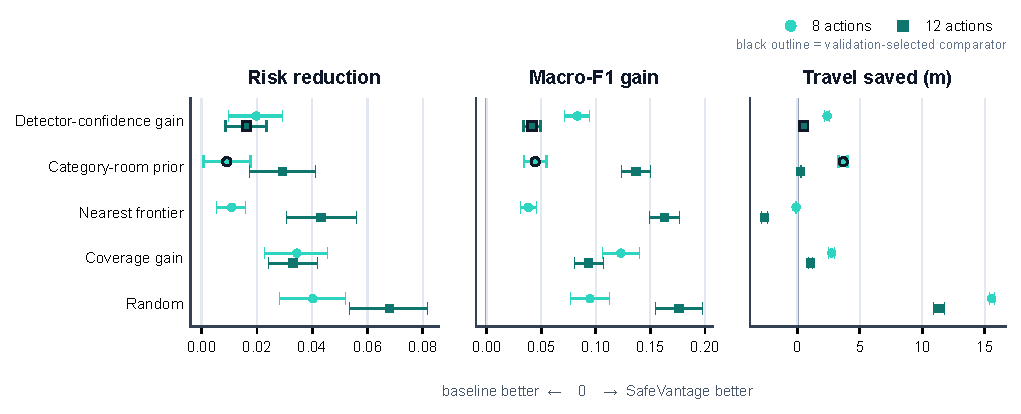
\includegraphics[width=\linewidth]{figures/fig_locked_all_baseline_forest_right_favorable_v2.pdf}
  %    \caption{\textbf{SafeVantage versus five equal-budget policies.} Points are paired differences; bars are 95\% scene-bootstrap intervals. Favorable values point left for risk/travel and right for macro-F1.}
  %    \label{fig:locked-forest}
   % \end{figure}
      %  Figure~\ref{fig:locked-forest} expands the comparison to all five baselines. \method{} ranks first in risk, macro-F1, and answer rate at both horizons, and travel is lower than four of five baselines. Nearest frontier travels 0.10~m less at eight actions and 2.63~m less at twelve, while \method{} improves macro-F1 by 0.0380/0.1630 and risk by 0.0109/0.0432.
    % Fig.~\ref{fig:locked-traces} further clarifies the entire process by following one held-out positive query from route selection to decision. Starting from the same pose with an 8-action budget, category-room prior travels 13.7~m without observing the queried paper towel and incorrectly returns \textsc{No}. In contrast, \method{} first obtains a partial detection, then reaches a target-visible viewpoint, and finally corroborates the detection from an additional position. It accumulates 4 supporting views, travels 5.4~m, and correctly returns \textsc{Yes}. 
    Fig.~\ref{fig:locked-traces} illustrates one held-out episode in which \method{} converts an initial partial detection into corroborated evidence and answers correctly while travelling less than the comparison policy.
    
    \begin{figure}[t]
      \centering
      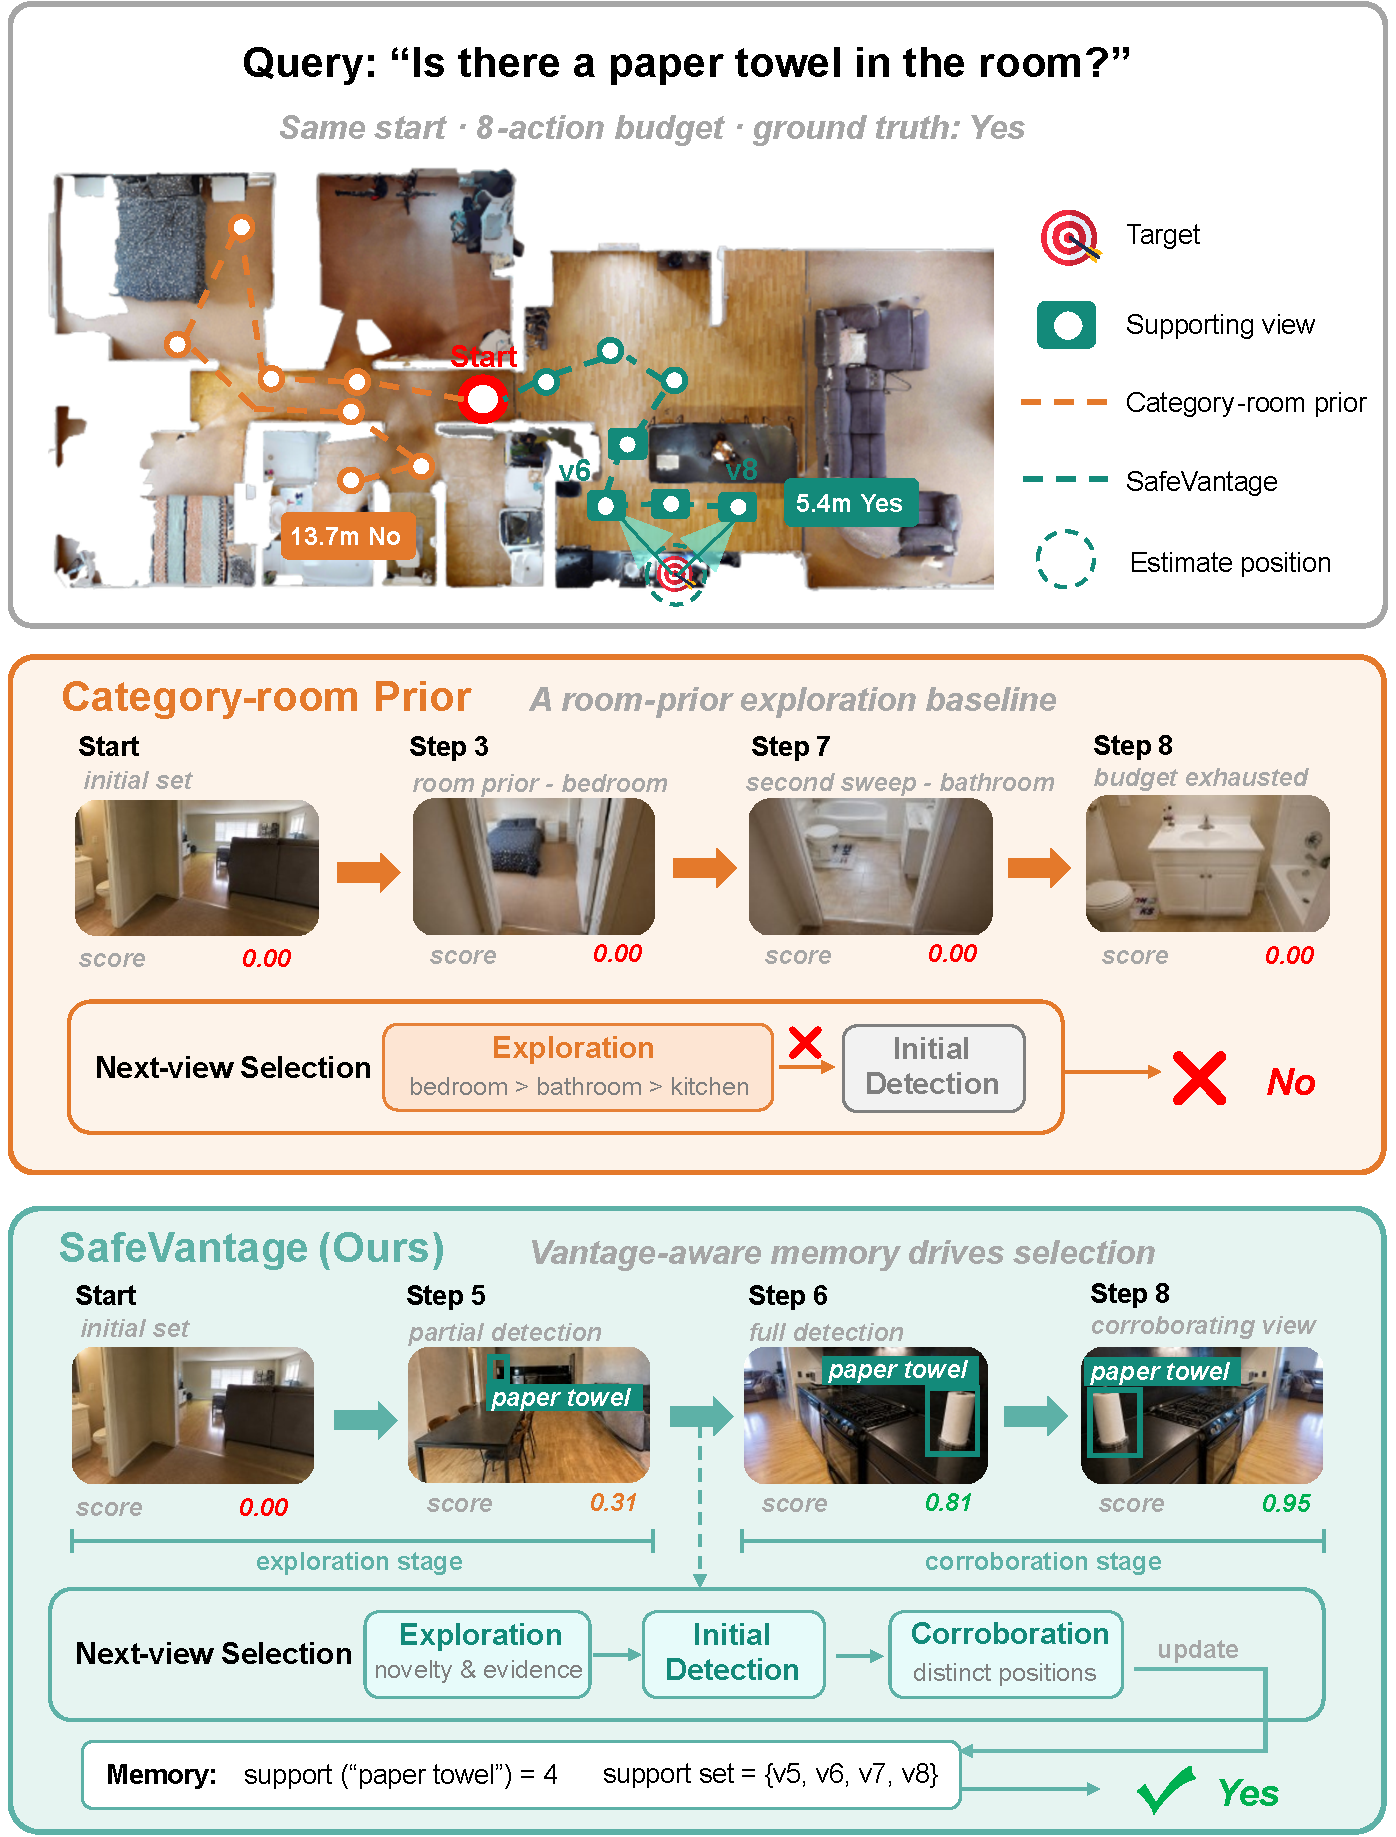
\includegraphics[width=\linewidth]{figures/zuyi_figure/example_v2.pdf}
      \caption{\textbf{One held-out episode for “Is there a paper towel in the room?”} Both policies start from the same start with an 8-action budget and a positive ground-truth label. Category–room prior does not observe the target, answers \textsc{NO}, and travels 13.7 m; \method{} acquires 4 supporting views, answers \textsc{YES}, and travels 5.4 m.}
      \label{fig:locked-traces}
    \end{figure}

    \begin{table*}[t]
    \centering
        \caption{
            Equal-input HM3D experiments. $R_9$ repeats calibration across nine folds; $R_{@\mathrm{cov}}$ matches coverage. Lower risk and AURC are better.
        }
        \label{tab:main}
    
        \small
        \renewcommand{\arraystretch}{1.15}
        \begin{tabular*}{\textwidth}{@{\extracolsep{\fill}}lrrrrrrrr@{}}
            \toprule
            Method
            & Cov.
            & Acc.
            & FP
            & Recall
            & Risk
            & $R_9$
            & $R_{@\mathrm{cov}}$
            & AURC \\
            \midrule
    
            \textbf{SafeVantage}
            & 0.436
            & \textbf{0.962}
            & \textbf{0.059}
            & 0.584
            & \textbf{0.524}
            & \textbf{0.538}
            & \textbf{0.538}
            & \textbf{0.649} \\
    
            Qwen2 caption-RAG
            & 0.565
            & 0.881
            & 0.240
            & \textbf{0.692}
            & 0.715
            & 0.638
            & 0.685
            & 0.715 \\
    
            ConceptGraphs
            & 0.432
            & 0.920
            & 0.123
            & 0.552
            & 0.617
            & 0.594
            & 0.707
            & 0.726 \\
    
            VLMaps
            & 0.541
            & 0.916
            & 0.162
            & 0.689
            & 0.618
            & 0.656
            & 0.910
            & 0.850 \\
    
            \bottomrule
        \end{tabular*}
    \end{table*}
    

    \subsection{Secondary Evidence in HM3D and ScanNet}
    
    Having tested the complete policy under the ProcTHOR benchmark, we conduct two secondary studies that examine supporting-view evidence under fixed observations and controlled interventions. On HM3D~\citep{yadav2023hm3dsem}, we compare semantic memory methods using identical RGB-D/pose inputs and a shared selective-decision rule. On ScanNet~\citep{dai2017scannet}, we remove and restore geometrically verified target-visible views while preserving the remaining input conditions, measuring their effect on downstream VLM answers.

    \textbf{Equal-input evaluation on HM3D.}
    % To evaluate the informativeness of viewpoint provenance under fixed observations, we compare \method{} with Qwen2 caption-RAG, ConceptGraphs, and released-code VLMaps on 36 HM3D-Sem scenes, using a 41-concept vocabulary and 1,436 category-presence queries labeled by Habitat semantics. Every method receives the same 160 RGB-D observations with camera poses per scene. \method{} uses Qwen2-VL-7B object lists~\citep{wang2024qwen2vl} and caption-RAG uses descriptions of all 5,760 input frames generated by the same model. ConceptGraphs and VLMaps process the same RGB-D/pose observations. We repeat calibration over nine disjoint 4-scene subsets, evaluating on the remaining 32 scenes in each repetition. At the minimum-risk setting, \method{} reaches 0.436 coverage, 0.962 answered accuracy, 0.059 false-positive rate, 0.584 recall, and 0.524 risk, compared with risks of 0.715, 0.617, and 0.618 for caption-RAG, ConceptGraphs, and VLMaps, respectively, which is shown in Table~\ref{tab:main}. Across nine 4-scene calibration folds, out-of-calibration risk $R_9$ is 0.538 for \method{}, compared with 0.638, 0.594, and 0.656, respectively. \method{} also has the lowest matched-coverage risk $R_{@\mathrm{cov}}$ and area under the risk–coverage curve (AURC). 
    We compare \method{}, Qwen2 caption-RAG, ConceptGraphs, and VLMaps on 36 HM3D-Sem scenes and 1,436 category-presence queries. Every method receives the same 160 RGB-D observations and camera poses per scene, with calibration repeated over nine disjoint 4-scene subsets. At the minimum-risk operating point, \method{} attains risk 0.524, versus 0.715, 0.617, and 0.618 for caption-RAG, ConceptGraphs, and VLMaps, and also the lowest out-of-calibration risk, matched-coverage risk, and AURC (Table~\ref{tab:main}).

   % \begin{table}[t]
   %   \centering
    %  \caption{\textbf{Equal-input HM3D experiments.} $R_9$ repeats calibration across nine folds; $R_{@\mathrm{cov}}$ matches coverage. Lower risk and AURC are better.}
    %  \label{tab:main}
    %  \resizebox{\linewidth}{!}{\begin{tabular}{lrrrrrrrr}
\toprule
method & cov. & acc. & FP & recall & risk & $R_{9}$ & $R_{@\mathrm{cov}}$ & AURC \\
\midrule
\textbf{SafeVantage} & 0.436 & \textbf{0.962} & \textbf{0.059} & 0.584 & \textbf{0.524} & \textbf{0.538} & \textbf{0.538} & \textbf{0.649} \\
Qwen2 caption-RAG & 0.565 & 0.881 & 0.240 & \textbf{0.692} & 0.715 & 0.638 & 0.685 & 0.715 \\
ConceptGraphs & 0.432 & 0.920 & 0.123 & 0.552 & 0.617 & 0.594 & 0.707 & 0.726 \\
VLMaps & 0.541 & 0.916 & 0.162 & 0.689 & 0.618 & 0.656 & 0.910 & 0.850 \\
\bottomrule
\end{tabular}
}
    %\end{table}
    
    \textbf{Supporting-view intervention on ScanNet.} To test whether supporting observations materially affect downstream answers, we conduct a controlled intervention on 73 ScanNet questions. Official instance geometry, camera poses, and depth determine whether the queried instance is visible, independently of the VLM reader. For each question, target-visible frames are replaced at their original ranks by target-absent frames while the question, reader, prompt configuration, input ranks, and history length remain fixed. Starting from this target-absent history, we restore the strongest supporting view, the strongest 4 views, or the complete original supporting-view set, thereby varying the available target evidence while preserving the input-history structure. As shown in Table~\ref{tab:causal}, Qwen2-VL token F1 increases from 0.2483 without target-visible views to 0.4410 with 4 restored views and 0.4540 with the complete set; Qwen2.5-VL improves from 0.1888 to 0.3215 under complete restoration. In a separate negative-decision diagnostic, we combine view-opportunity and source-group coverage with evidence scores, calibrating the threshold on 6 development scenes under a 5\% false-negative-decision constraint and evaluating on 12 held-out ScanNet scenes. The rule achieves 0.983 observed-absent recall and 0.935 negative-decision precision, versus 0.051 and 0.500 for a score-only rule, with a 0.033 erroneous-negative-decision rate over non-absent states. Together, these results show that supporting views improve downstream answers, while coverage helps distinguish observed absence from unresolved missing evidence.

    \begin{table}[t]
      \centering
      \caption{ScanNet supporting-view intervention. Intervals compare restored conditions with target-absent histories.}
      \label{tab:causal}
      \small
      \setlength{\tabcolsep}{2pt}
      \renewcommand{\arraystretch}{1.18}
      \begin{tabular}{llccc}
\toprule
reader & evidence set & F1 & $\Delta$ vs absent & scene CI \\
\midrule
Qwen2-VL & target absent & 0.2483 & -- & -- \\
Qwen2-VL & strongest 1 & 0.3565 & +0.1082 & [-0.0181, 0.2290] \\
Qwen2-VL & strongest 4 & 0.4410 & +0.1927 & [0.0691, 0.2977] \\
Qwen2-VL & complete & \textbf{0.4540} & \textbf{+0.2057} & \textbf{[0.0752, 0.3133]} \\
Qwen2.5-VL & target absent & 0.1888 & -- & -- \\
Qwen2.5-VL & complete & 0.3215 & +0.1327 & [0.0513, 0.2053] \\
\bottomrule
\end{tabular}


      
    \end{table}


    \begin{figure}[t]
      \centering
      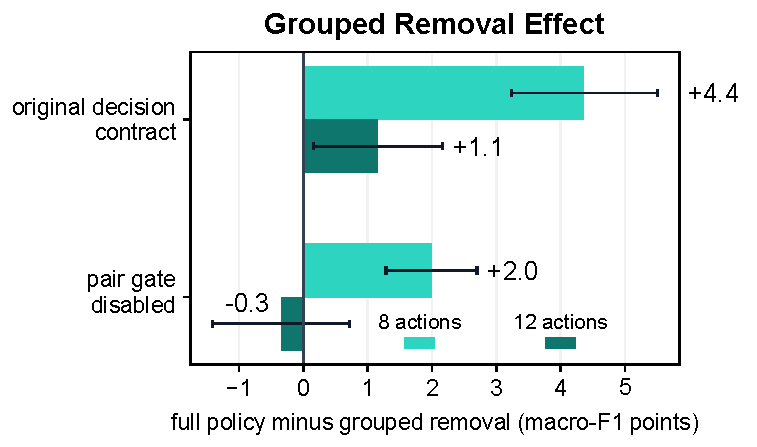
\includegraphics[
        width=\linewidth,
        height=0.25\textheight,
        keepaspectratio
      ]{figures/zuyi_figure/Fig_4.pdf}
      \caption{\textbf{Removing vantage-aware state lowers macro-F1.} Bars show full policy minus grouped removal on 96 validation houses; whiskers are paired 95\% intervals.}
      \label{fig:grouped-vantage}
    \end{figure}

\begin{table}[b]
  \centering
   \caption{Component ablations on 96 ProcTHOR validation houses. Loss is the macro-F1 drop from the full model (pp).}
  \label{tab:component-validation}

  \small
  \setlength{\tabcolsep}{2pt}
  \renewcommand{\arraystretch}{1.18}

  \begin{tabular*}{\columnwidth}{@{\extracolsep{\fill}}lcccc@{}}
  \toprule
  & \multicolumn{2}{c}{8 actions}
  & \multicolumn{2}{c}{12 actions} \\
  \cmidrule(lr){2-3}\cmidrule(l){4-5}

  Variant
  & F1$\uparrow$ & Loss (pp)$\downarrow$
  & F1$\uparrow$ & Loss (pp)$\downarrow$ \\
  \midrule

  \textbf{Full \method{}}
  & \textbf{0.5307} & --
  & \textbf{0.6149} & -- \\

  $-$ claim provenance
  & 0.4753 & \textbf{+5.54}
  & 0.5826 & \textbf{+3.23} \\

  $-$ target-ray alignment
  & 0.4749 & \textbf{+5.58}
  & 0.5819 & \textbf{+3.30} \\

  $-$ yaw diversity
  & 0.5311 & $-0.04$
  & 0.6162 & $-0.13$ \\

  $-$ base geometry
  & 0.5255 & \textbf{+0.52}
  & 0.6167 & $-0.18$ \\

  $-$ directed exploration
  & 0.5247 & \textbf{+0.60}
  & 0.4923 & \textbf{+12.26} \\

  \addlinespace[2pt]
  Confidence backbone only
  & 0.4847 & \textbf{+4.60}
  & 0.4835 & \textbf{+13.14} \\

  \bottomrule
\end{tabular*}
\end{table}
    
    \subsection{Ablations}

    We finally examine which acquisition components contribute to decision quality and how their effects depend on the final evidence gate. All variants are evaluated on 96 query-eligible ProcTHOR validation houses at 8- and 12-action budgets under a shared 20~m travel cap, yielding 3,072 paired episodes per variant and budget.

    % \textbf{Grouped removal.} To test the mechanism directly, we first jointly remove supporting-view identity, target-ray alignment, and yaw diversity from candidate-view selection while retaining room evidence, coverage features, base geometry, and the travel objective. Macro-F1 decreases by 4.35 points at 8 actions and 1.15 points at 12 actions, with 95\% confidence intervals of $[3.23,5.50]$ and $[0.16,2.16]$, respectively. This establishes a joint contribution under the original decision rule.  Besides, we repeat the comparison with the pair gate disabled in both policies. This gate requires geometrically consistent target estimates from two distinct supporting positions before a positive commitment. Fig.~\ref{fig:grouped-vantage} reports the grouped removal results. 

    \textbf{Grouped removal.} Jointly removing supporting-view identity, target-ray alignment, and yaw diversity (retaining room evidence, coverage, base geometry, and the travel objective) lowers macro-F1 by 4.35/1.15 points at 8/12 actions (95\% CIs $[3.23,5.50]$/$[0.16,2.16]$; Fig.~\ref{fig:grouped-vantage}). The effect persists with the pair gate disabled in both policies, separating acquisition from decision-time consistency.

    \textbf{Candidate observability.}
    Removing the candidate-observability model while holding the remaining
    controller fixed lowers macro-F1 by 7.52 and 8.03 points at 8 and
    12 actions, respectively. Mean travel simultaneously increases from
    4.94 to 6.30~m and from 7.44 to 8.95~m. So, candidate observability
    improves both decision quality and acquisition efficiency across both
    action horizons.
    
    \textbf{Component contributions.} Table~\ref{tab:component-validation} reports 5 single-component removals and a confidence-backbone-only variant. Removing supporting-view identity or target-ray alignment reduces macro-F1 by 5.54/3.23 and 5.58/3.30 points at 8/12 actions, respectively. Directed exploration has a strongly budget-dependent contribution: removing it costs 0.60 points at 8 actions but 12.26 points at 12 actions. Retaining only the confidence backbone loses 4.60/13.14 points. Other geometric terms show smaller or inconsistent marginal effects.
    
    % further showing the importance of the additional acquisition mechanisms at the longer horizon. Removing yaw diversity produces small increases in the F1 point estimates, while removing base geometry yields mixed changes across budgets. These results do not establish consistent individual gains for either term.

\subsection{Evaluation on a Disjoint Holdout}

To test generalization beyond the original 232-house evaluation, we held the method, thresholds, and evaluator fixed and tested on a disjoint cohort of 233 additional ProcTHOR houses that were never used for training, validation, or the original evaluation. On this cohort, \method{} improves macro-F1 by 7.3 and 4.3 points at 8 and 12 actions, respectively (95\% paired scene-bootstrap intervals $[6.4,8.1]$ and $[3.3,5.2]$). Risk decreases by 0.024 and 0.015, respectively, with higher answer rate and
lower travel at both horizons. These results confirm that the
acquisition advantage transfers to unseen houses.   

   
    
\section{Limitations}

Our study focuses on category-presence queries, providing a controlled setting for examining the role of viewpoint evidence. Extending this formulation to attributes, relations, and temporal changes may require richer representations of evidence sufficiency. The acquisition policy uses a fixed perception stack and a candidate-observability model, with observations selected from a discrete viewpoint graph under fixed action budgets. Robustness to changes in perception and sensing conditions therefore remains an area for further evaluation. While the HM3D and ScanNet studies provide complementary evidence analyses, continuous navigation and real-robot evaluation are natural next steps toward assessing the framework under broader operating conditions.


\section{Conclusion}

In this work, we addressed the problem of acquiring sufficient visual evidence for reliable embodied decisions under partial observability. We introduced \method{}, a vantage-aware semantic memory that retains each claim's supporting views and target geometry while keeping positive support distinct from search coverage. This retained vantage evidence is what enables the rest of the system: it grounds the learned candidate-observability model, drives view selection by expected reduction in decision loss, and, through a geometric consistency gate, calibrated \textsc{Yes}/\textsc{No}/\textsc{Abstain} decisions. Experiments on held-out ProcTHOR houses show higher macro-F1 and answer rates with lower risk and travel than the validation-selected equal-budget baselines at both action horizons. Complementary HM3D comparisons demonstrate lower selective risk under identical observations, while ScanNet interventions show that restoring supporting views improves downstream VLM answers. Ablations further support the contributions of candidate observability and claim provenance. Together, these results support treating memory as an evidence state that guides both observation acquisition and semantic commitments, rather than solely as a representation for retrieval.
% Future work will extend this approach to attributes, relations, and temporal changes, and evaluate evidence-guided acquisition under continuous control and real-robot sensing.

\section{Acknowledgments}
The authors used generative AI tools during manuscript preparation to assist with generating and revising selected text and figures, as well as code generation and debugging.
    
   % \textbf{Limitations.}
   % Our current evaluation focuses primarily on category-presence queries in simulated indoor environments, using a fixed perception stack and a discrete viewpoint action graph. These settings do not fully capture detector shift, continuous control, or real-world sensing noise. In addition, attributes, relations, temporal changes, and manipulation preconditions may require richer notions of evidence sufficiency than viewpoint support alone. Future work will extend SafeVantage toward question-conditioned evidence acquisition, continuous control, and real-robot evaluation.
    
   % \textbf{Societal Impact.}
   % SafeVantage aims to improve the reliability and auditability of embodied agents by reducing unsupported semantic commitments and exposing the visual evidence behind a decision. Potential applications include household robots, inspection systems, and assistive agents. Practical deployment, however, should account for sensor and environment shift, privacy of captured observations, appropriate risk calibration, and safe fallback behavior when evidence remains insufficient.
    
    % ICRA / IEEE bibliography style
    \bibliographystyle{IEEEtran}
    \bibliography{references}
    
    \clearpage
   % \appendix
    
   % \section{Reproducibility and Experimental Protocol}
   % \label{app:contract}
    %\subsection{ProcTHOR Split and Frozen Evaluation}
   % \label{app:fresh-active}
   % The primary benchmark uses official ProcTHOR-10K splits, a training-derived 24-category vocabulary, 160 candidate viewpoints per scene, exact geodesic costs, and a 20-m travel cap. Of 256 held-out identities, 255 materialize; balanced-query construction yields 232 scenes and 7,424 paired episodes per method and action budget. Scene identities, detector predictions, action graphs, starts, queries, acquisition parameters, and decision heads are fixed before test evaluation. Policies never receive simulator instance identity or hidden visibility. The combiner requires identical $(\mathrm{scene},\mathrm{category},\mathrm{start},\mathrm{budget})$ keys and rejects duplicates before 10,000-draw paired whole-scene bootstrap analysis.
    
    %At eight actions, the frozen policy uses low-cost exploration, travel exponent 2.0, a 1.50-m edge cap, detection trigger 0.15, and ray weight 8.0; its positive/negative probabilities are 0.85/0.30 with support threshold 0.10 and 1.0-m pair radius. At twelve actions, it uses coverage exploration, exponent 3.0, a 0.75-m edge cap, trigger 0.10, and ray weight 2.0; the decision values are 0.40/0.30, support threshold 0.30, and the same pair radius. Both policies execute the complete horizon.
    
   % The comprehensive test adds training-only heads for random, nearest frontier, coverage gain, category--room prior, and detector-confidence gain while importing the byte-equivalent frozen \method{} model. It changes no scene, query, detector prediction, acquisition action, \method{} probability, or threshold.
    
    %The selected settings are Pareto-optimal in the 72-policy training archive. All six one-factor neighbors at each horizon retain joint improvements in risk, macro-F1, and travel.
    
    %\subsection{Complementary 3D Protocols}
   % The HM3D comparison fixes 36 scenes, a 41-concept vocabulary, and the same 160 RGB-D/pose observations per scene for every method. Its separate 1024-view semantic sweep is descriptive and excluded from scores. Each method exposes one scalar score per query and receives the same two-threshold adapter. Nine disjoint four-scene calibration folds evaluate the remaining 32 scenes. Qwen2-VL-7B captions all 5,760 frames for caption-RAG; ConceptGraphs and VLMaps use those same RGB-D/pose frames. An independent 8,628-row reconstruction verifies \method{} support counts and source-view identities.
    
    %For ScanNet, official instance geometry, camera pose, and depth determine whether the queried instance is visible. Target-visible frames are replaced at the same ranks by target-absent frames while history length, reader, prompt family, and question stay fixed. The complete condition restores the original supporting views; intervals cluster by scene. For the active HM3D diagnostic, 12 scene identifiers, 1,097 episodes, candidates, outputs, and two seeds are frozen. Candidates on disconnected navmesh islands are removed before scoring, and every displayed camera is an executed action from the metric candidate set.
    
    %\subsection{Compute and Artifacts}
   % Learned detector and VLM predictions are generated once on single-GPU L40S, H100, or H200 shards and cached. Policy replay and uncertainty analyses are CPU-parallel. The component audit uses 56 four-CPU, 24-GB tasks capped at three hours; the grouped intervention uses 32 four-CPU, 24-GB tasks capped at two hours. Machine-readable results, row hashes, launchers, analysis code, and figure generators accompany the source bundle.
    
    % \section{Held-Out ProcTHOR Diagnostics}
    % \subsection{Trajectory Gallery}
    % \label{app:locked-traces}
    % Figure~\ref{fig:locked-gallery} expands the main-paper episode to six held-out cases spanning positive recovery, false-positive avoidance, absence resolution, and travel reduction. Each row joins the occupancy-map route to observations sampled from the policy history. Orange and teal paths begin from the same start and use the same action graph.
    
    % \begin{figure}[p]
    %   \centering
    %   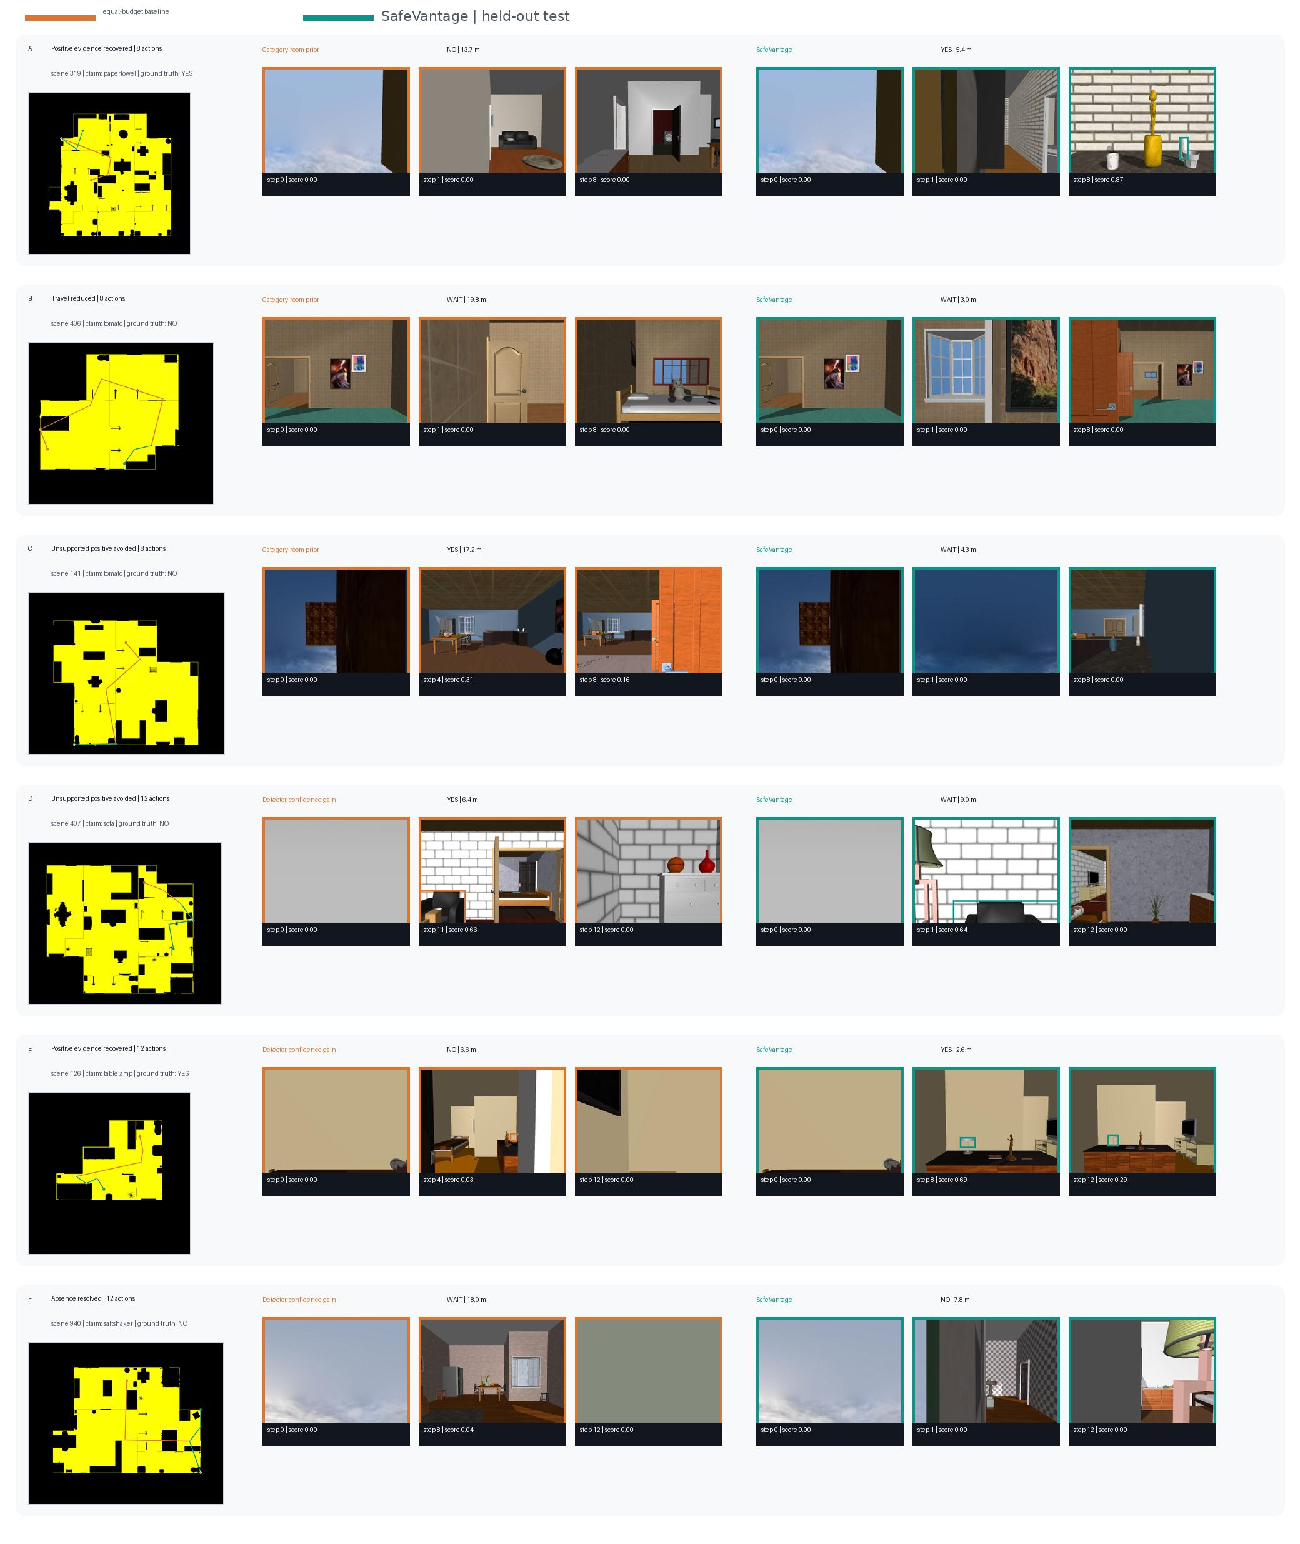
\includegraphics[width=\linewidth,height=0.84\textheight,keepaspectratio]{figures/fig_locked_trajectory_gallery.pdf}
    %   \caption{\textbf{Six held-out acquisition-to-decision traces.} The gallery covers recovered evidence, avoided false positives, efficient \textsc{Abstain}, and resolved absence at both action budgets.}
    %   \label{fig:locked-gallery}
    % \end{figure}
    % \FloatBarrier
    
    % \subsection{Category Breakdown}
    % \label{app:category-diagnostics}
    % Aggregate superiority need not be uniform across categories. Figure~\ref{fig:category-heatmap} compares \method{} with the primary baseline at each budget. Most category cells favor \method{}, and travel savings are broad at eight actions. The visible red cells are equally important: for example, twelve-action countertop macro-F1 is worse despite the aggregate win. These cells are descriptive slices with fewer episodes, not separately powered hypothesis tests.
    
    % \begin{figure}[H]
    %   \centering
    %   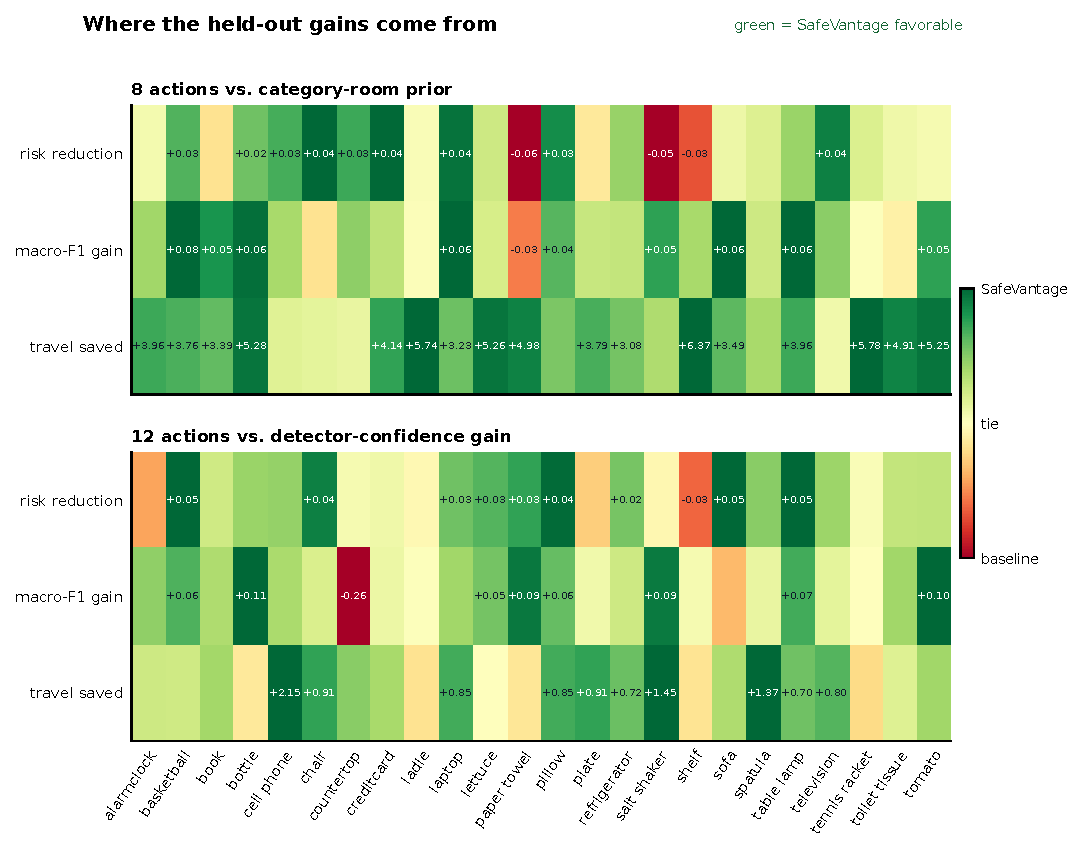
\includegraphics[width=\linewidth]{figures/fig_locked_category_heatmap.pdf}
    %   \caption{\textbf{Category-level held-out effects.} Green favors \method{}; rows show risk reduction, macro-F1 gain, and travel saved at each budget.}
    %   \label{fig:category-heatmap}
    % \end{figure}
    
   % \section{Cross-Environment Evidence Studies}
   % \subsection{Equal-Input HM3D Operating Points}
    %Table~\ref{tab:main} reports the complete held-out HM3D ledger under one decision wrapper. All methods receive the same 160 RGB-D/pose frames.
    
    
    
   % At the minimum-risk setting, \method{} reaches 0.436 coverage, 0.962 answered accuracy, 0.059 false-positive rate, and 0.524 risk. Its absolute risk reduction is 0.191 [0.130, 0.254] against caption-RAG, 0.094 [0.047, 0.142] against ConceptGraphs, and 0.099 [0.051, 0.148] against equal-view VLMaps. Across nine four-scene calibration folds, mean out-of-calibration risk is 0.538 for \method{}, 0.594 for ConceptGraphs, 0.638 for caption-RAG, and 0.656 for VLMaps; \method{} also has the lowest matched-coverage risk and AURC.
    
   % \subsection{ScanNet Supporting-View Intervention}
    %The ScanNet intervention keeps question, reader, prompt, rank, and history length fixed while changing only whether depth-verified target views occupy the selected ranks. Table~\ref{tab:causal} reports both readers and scene-clustered intervals against the target-absent condition.
    
   % \begin{table}[H]
   %   \centering
   %   \caption{\textbf{ScanNet supporting-view intervention.} Intervals compare each restored condition with target-absent histories.}
   %  \label{tab:causal}
     % \begin{adjustbox}{max width=\columnwidth,max height=0.35\textheight}
        %\begin{tabular}{llccc}
\toprule
reader & evidence set & F1 & $\Delta$ vs absent & scene CI \\
\midrule
Qwen2-VL & target absent & 0.2483 & -- & -- \\
Qwen2-VL & strongest 1 & 0.3565 & +0.1082 & [-0.0181, 0.2290] \\
Qwen2-VL & strongest 4 & 0.4410 & +0.1927 & [0.0691, 0.2977] \\
Qwen2-VL & complete & \textbf{0.4540} & \textbf{+0.2057} & \textbf{[0.0752, 0.3133]} \\
Qwen2.5-VL & target absent & 0.1888 & -- & -- \\
Qwen2.5-VL & complete & 0.3215 & +0.1327 & [0.0513, 0.2053] \\
\bottomrule
\end{tabular}


    %  \end{adjustbox}
   % \end{table}
    
    % \subsection{HM3D Resolving-View Trace}
    % \label{app:hm3dtraces}
    % Figure~\ref{fig:active_trace} is the qualitative counterpart to the matched-cost selector result. Geometry and the 2D map choose 1.5-m actions that reveal zero queried-category pixels. The 3D evidence selector chooses a reachable 2.6-m geodesic action that reveals 419 vase pixels. Every candidate lies on the source navmesh component, and the mesh, path, rendered observation, semantic pixels, and decision ledger come from the same episode.
    
    % \begin{figure}[H]
    %   \centering
    %   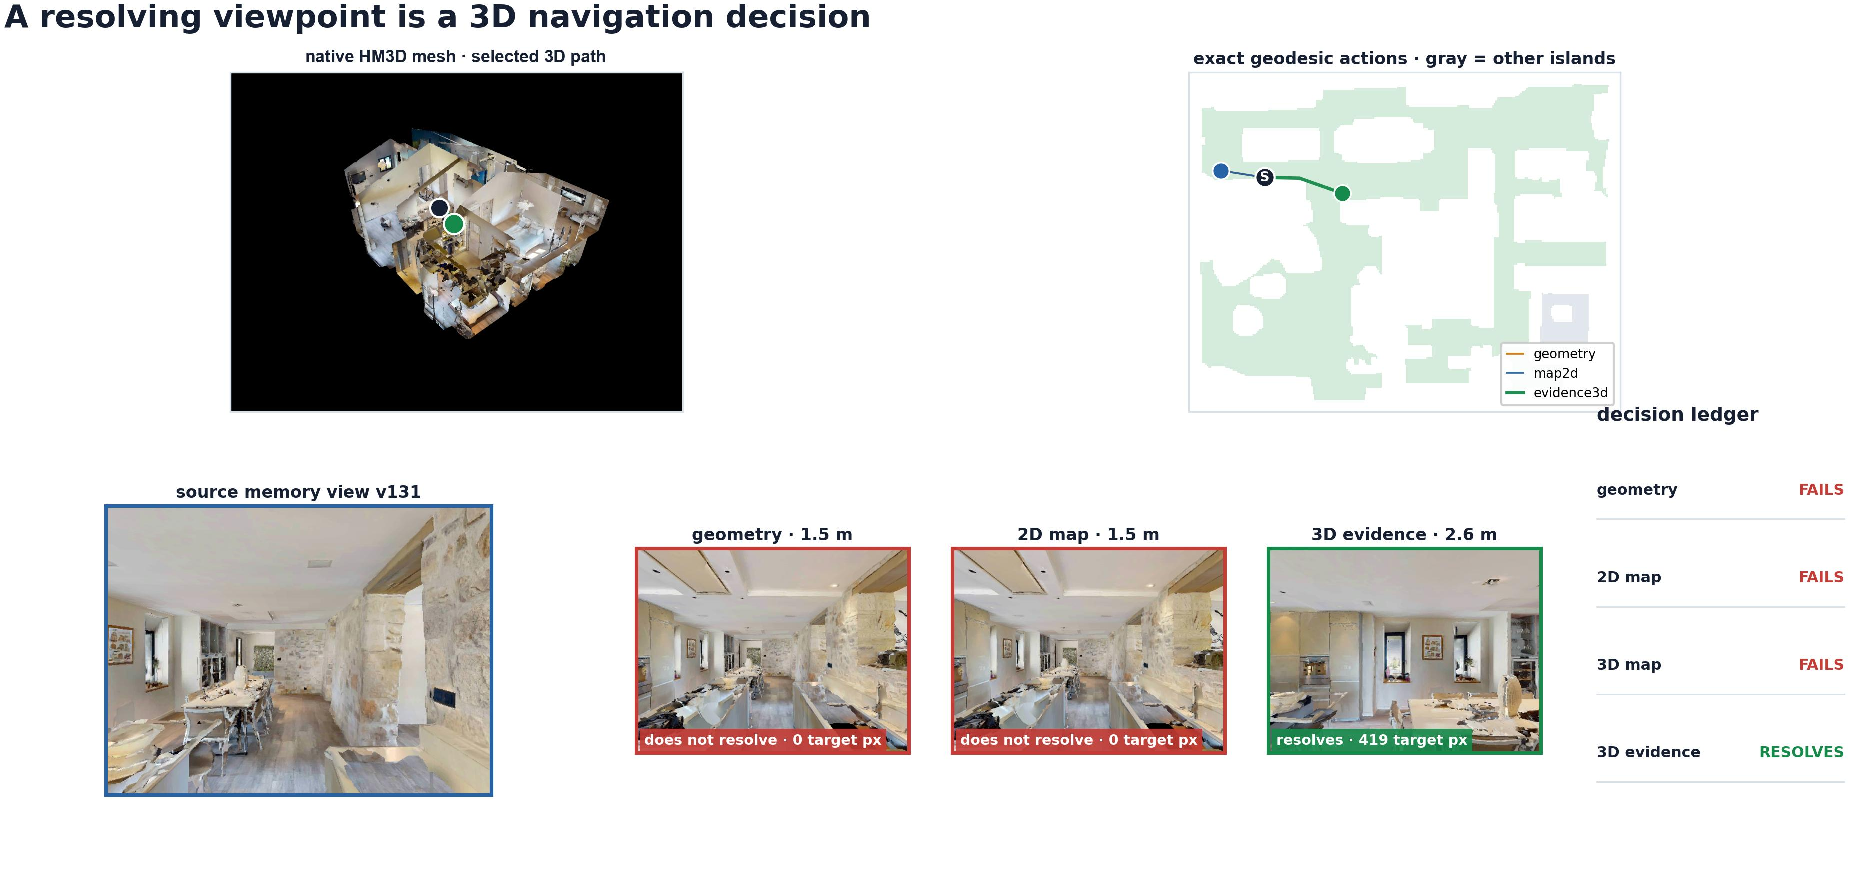
\includegraphics[width=\linewidth,height=0.84\textheight,keepaspectratio]{figures/fig50_hm3d_active_trace.pdf}
    %   \caption{\textbf{An HM3D resolving-view trace.} Evidence-3D reveals 419 vase pixels from a reachable view missed by equal-budget geometry and 2D-map selectors.}
    %   \label{fig:active_trace}
    % \end{figure}
    % \FloatBarrier
    
   % \section{Mechanism and Robustness}
    % \subsection{Matched Component Audit}
    % \label{app:component-audit}
    % The component audit uses 116 ProcTHOR training scenes and 3,712 paired episodes per variant and budget. Each variant reruns acquisition, keeps the feature schema fixed, and refits the same selective-head architecture with scene-disjoint folds. The full-controller row reproduces the previously frozen training histories; row hashes are included in the artifact bundle.
    
    % Table~\ref{tab:component-audit} gives the complete seven-variant ledger. Removing supporting-view identity or target-ray alignment lowers macro-F1 by 0.0565 at eight actions and about 0.0322 at twelve. Directed exploration is the long-horizon term: removing it lowers macro-F1 by 0.1345 and raises risk by 0.0373 at twelve actions. The confidence-backbone-only controller loses 0.0469/0.1615 macro-F1 at eight/twelve actions; yaw diversity and base geometry have smaller effects.
    
    % \begin{table}[H]
    %   \centering
    %   \caption{\textbf{Train-OOF component audit.} Each removal reruns acquisition and refits the same scene-disjoint head on 116 scenes.}
    %   \label{tab:component-audit}
    %   \begin{adjustbox}{max width=\columnwidth,max height=0.35\textheight}
    %   \scriptsize
    %   \resizebox{\linewidth}{!}{\begin{tabular}{@{}lccc ccc@{}}
  \toprule
  & \multicolumn{3}{c}{8 actions} & \multicolumn{3}{c}{12 actions} \\
  \cmidrule(lr){2-4}\cmidrule(l){5-7}
  Variant & Risk$\downarrow$ & F1$\uparrow$ & Travel$\downarrow$ & Risk$\downarrow$ & F1$\uparrow$ & Travel$\downarrow$ \\
  \midrule
  \textbf{Full \method{}} & \textbf{0.3799} & \textbf{0.5712} & \textbf{2.89} & \textbf{0.3312} & \textbf{0.6736} & \textbf{6.29} \\
  $-$ claim provenance & 0.3940 & 0.5148 & 2.88 & 0.3510 & 0.6414 & 6.28 \\
  $-$ target-ray alignment & 0.3940 & 0.5148 & 2.88 & 0.3510 & 0.6413 & 6.28 \\
  $-$ yaw diversity & 0.3806 & 0.5706 & 2.90 & 0.3292 & 0.6744 & 6.29 \\
  $-$ base geometry & 0.3828 & 0.5617 & 3.05 & 0.3321 & 0.6714 & 6.29 \\
  $-$ directed exploration & 0.3847 & 0.5608 & 2.86 & 0.3685 & 0.5391 & 4.36 \\
  Confidence backbone only & 0.3892 & 0.5243 & 2.85 & 0.3808 & 0.5121 & 4.36 \\
  \bottomrule
\end{tabular}
}
    %   \end{adjustbox}
    % \end{table}
    
   % \subsection{Train-Frozen Validation Confirmation}
    %The seven variants are applied to 96 query-eligible validation houses with acquisition settings and train-fitted heads held fixed, yielding 3,072 paired episodes per row and budget. The full controller reaches macro-F1 0.5307/0.6149 at eight/twelve actions. Removing supporting-view identity loses 5.54/3.23 points; removing target-ray alignment loses 5.58/3.30. Directed exploration is the long-horizon term, losing 12.26 points at twelve actions, while the confidence backbone loses 13.14.
    
    
    
    % \begin{figure}[H]
    %   \centering
    %   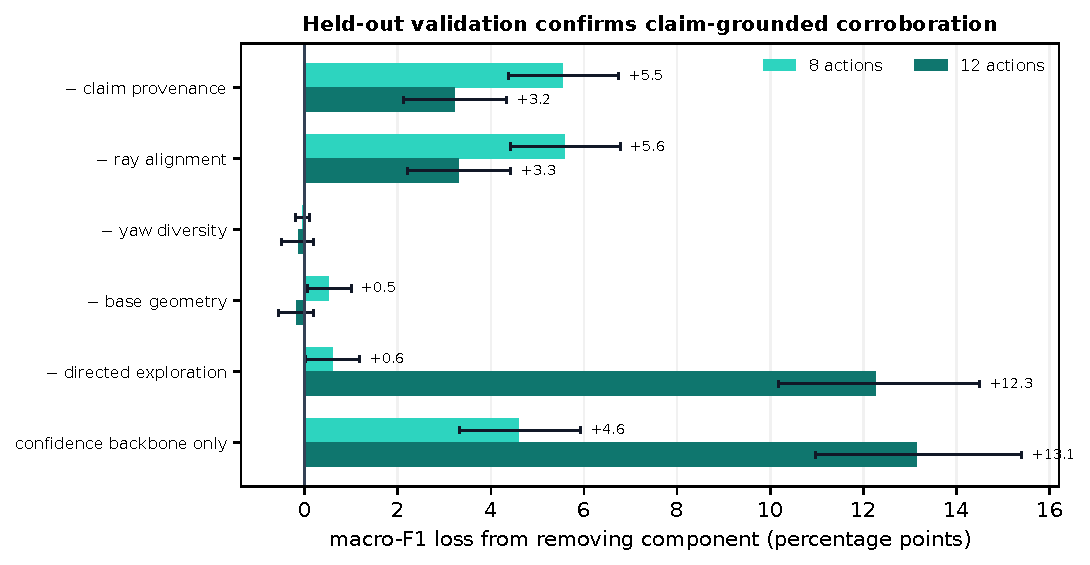
\includegraphics[width=\linewidth]{figures/fig_component_validation.pdf}
    %   \caption{\textbf{Component effects transfer to validation.} Bars are macro-F1 losses from train-frozen removals; whiskers are paired 95\% scene-bootstrap intervals.}
    %   \label{fig:component-validation}
    % \end{figure}
    
   % \subsection{Robustness and Deployment Scope}
   % \label{app:robustness}
   % \textbf{Negative decisions.} Positive support and search coverage are complementary. A coverage measure uses the fraction of sampled view opportunities and source groups already observed, together with existing evidence scores. Its threshold is selected on six development scenes under a 5\% false-negative-decision constraint and evaluated on 12 held-out ScanNet scenes. It attains 0.983 observed-absent recall, 0.935 negative-decision precision, and 0.033 false decisions over non-absent states; a score-only low-confidence rule attains 0.051 absent recall and 0.500 precision.
    
   % \textbf{Correlated support.} Nearby frames can repeat the same observation. Pose clustering leaves the HM3D ranking stable in our control. In the active-policy audits, removing supporting-view identity or target-ray alignment lowers macro-F1 at both horizons in training OOF and train-frozen validation.
    
   % \textbf{Independent-view causal control.} The ten-case equal-count pilot is retained as a reader-side composition control. In the larger ScanNet study, answer quality changes as supporting views are removed and restored; the active-policy ablation separately measures their acquisition value.
    
   % \textbf{Acquisition--decision interface.} The HM3D traces separate whether a selector finds a resolving view from how a downstream wrapper uses it. The primary ProcTHOR experiment evaluates both stages end to end.
    
    %\textbf{Detector and action-graph dependence.} The ProcTHOR comparison uses fixed YOLO-World predictions on discrete viewpoints, so the policies differ in acquisition rather than detector outputs. Detector-shift controls and continuous robot execution are the next deployment tests.
    
    %\textbf{Cost sensitivity.} The headline risk uses $(C_{\mathrm{FP}},C_{\mathrm{FN}},C_{\mathrm{A}})=(5,2,0.5)$. We evaluate an 18-cell grid with false-positive costs $\{1,2,3,5,8,10\}$ and abstention costs $\{0.25,0.5,1\}$, refitting the two-threshold adapter on the same calibration scenes in every cell. At FP cost 5 and abstention cost 0.5, scene-macro risk favors \method{} over caption-RAG by 0.192 [0.129, 0.256], ConceptGraphs by 0.094 [0.047, 0.141], and equal-160-view VLMaps by 0.099 [0.052, 0.147]. At FP cost 10, the corresponding gains are 0.445 [0.324, 0.576], 0.185 [0.086, 0.280], and 0.251 [0.152, 0.352]. Across all cells, \method{} wins 12, 14, and 11 comparisons, respectively.
    
    % NeurIPS-specific checklist is not part of the ICRA manuscript format.
    % \clearpage
    % \input{checklist}
    
    \end{document}
    